\documentclass[english]{kththesis}

\usepackage[style=numeric,sorting=none,backend=biber]{biblatex}
\usepackage[acronym, section=section, nonumberlist, nomain, nopostdot]{glossaries}
\usepackage[perpage,symbol]{footmisc}
\usepackage[parfill]{parskip} % Linebreak paragraphs instead of indent

\usepackage{longtable}
\usepackage{booktabs}
\usepackage{enumitem}

\usepackage{xcolor}     % Remove after \todo has been removed
\usepackage{tabularx}   % For additional table formatting
\usepackage{subcaption} % For subfigure support
\usepackage{pgfmath}    % --math engine
\usepackage{array}      % For table wrapping
\usepackage{graphicx}   % Support for images
\usepackage{float}      % Support for more flexible floating box positioning
\usepackage{setspace}   % For fine-grained control over line spacing
\usepackage{listings}   % For source code listing
\usepackage{tabularx}   % For simple table stretching
\usepackage{multirow}   % Support for multirow colums in tables
\usepackage{url}        % Support for breaking URLs
\usepackage{hyperref}
\usepackage[all]{hypcap}  % prevents an issue related to hyperref and caption linking
%% setup hyperref to use the darkblue color on links
\hypersetup{colorlinks,breaklinks,
            linkcolor=darkblue,urlcolor=darkblue,
            anchorcolor=darkblue,citecolor=darkblue}

%% Some definitions of used colors
\hyphenpenalty=15000\tolerance=1000 % to reduce hyphenation
\definecolor{darkblue}{rgb}{0.0,0.0,0.3} %% define a color called darkblue
\definecolor{darkred}{rgb}{0.4,0.0,0.0}
\definecolor{red}{rgb}{0.7,0.0,0.0}
\definecolor{lightgrey}{rgb}{0.8,0.8,0.8} 
\definecolor{grey}{rgb}{0.6,0.6,0.6}
\definecolor{darkgrey}{rgb}{0.4,0.4,0.4}
\definecolor{aqua}{rgb}{0.0, 1.0, 1.0}

\usepackage[cache=false]{minted} %% For source code highlighting
\usemintedstyle{borland}

\usepackage{csquotes} % Recommended by biblatex

% set the chapter header
\renewcommand{\chaptermark}[1]{\markboth{#1}{}}

% to get rolling footnote numbers
\counterwithout{footnote}{chapter}

\newcolumntype{P}[1]{>{\endgraf\vspace*{-\baselineskip}}p{#1}}

% custom macros
\newcommand{\footnotelink}[2]{\footnote{\url{#1} | Accessed #2}}
\newcommand{\todo}[0]{\colorbox{orange}{TODO}}

% The list of acronyms and abbreviations should be in alphabetical order based on the spelling of the acronym or abbreviation.
\makeglossaries

\newacronym{IOT}{IoT}{Internet of Things}

\date{\today}
\title{Ethical Hacking of Securitas' Home Alarm System}
% \subtitle{[Todo subtitle]}
\alttitle{Etisk Hackning av Securitas hemlarmsystem}
% \altsubtitle{[Todo subtitle]}

\authorsLastname{Lindeberg}
\authorsFirstname{Axel}
\email{alindeb@kth.se}
\kthid{alindeb}
\authorsSchool{\schoolAcronym{EECS}}
\programcode{CDATE}

% KTH Supervisor
\supervisorAsLastname{Johnson}
\supervisorAsFirstname{Pontus}
\supervisorAsEmail{pontusj@kth.se}
\supervisorAsKTHID{pontusj}
\supervisorAsSchool{\schoolAcronym{EECS}}
\supervisorAsDepartment{Division of Network and Systems Engineering}

% KTH Examiner
\examinersLastname{Lagerström}
\examinersFirstname{Robert}
\examinersEmail{robertl@kth.se}
\examinersKTHID{robertl}
\examinersSchool{\schoolAcronym{EECS}}
\supervisorAsDepartment{Division of Network and Systems Engineering}

% External Supervisor
%\supervisorBsLastname{[EFTERNAMN]}
%\supervisorBsFirstname{[NAMN]}
%\supervisorBsEmail{temp@fm.se}
%\supervisorBsOrganization{Försvarsmakten}
\hostcompany{Försvarsmakten (Swedish Armed Forces)}

\addbibresource{references.bib}

\begin{document}

\titlepage
\bookinfopage

\frontmatter
\setcounter{page}{1}

% ---- English Abstract ----
\begin{abstract}
\markboth{\abstractname}{}
% Keep in mind that most of your potential readers are only going to read your title and abstract. This is why it is important that the abstract give them enough information that they can decide is this document relevant to them or not. Otherwise the likely default choice is to ignore the rest of your document.
% A abstract should stand on its own, i.e., no citations, cross references to the body of the document, acronyms must be spelled out, …
% Write this early and revise as necessary. This will help keep you focused on what you are trying to do.

% Write an abstract (250 and 350 words) with the following components:
%  - What is the topic area? (optional) Introduces the subject area for the project.
%  - Short problem statement
%  - Why was this problem worth a Master’s thesis project? (i.e., why is the problem both significant and of a suitable degree of difficulty for a Master’s thesis project? Why has no one else solved it yet?)
%  - How did you solve the problem? What was your method/insight?
%  - Results/Conclusions/Consequences/Impact: What are your key results/conclusions? What will others do based upon your results? What can be done now that you have finished - that could not be done before your thesis project was completed? The presentation of the results should be the main part of the abstract.
\todo

\subsection*{Keywords}
% Choosing good keywords can help others to locate your paper, thesis, dissertation, … and related work.}
% Choose the most specific keyword from those used in your domain, see for example:
% ACM's Computing Classification System (2012) or
% (2014) IEEE Taxonomy. 
% Mechanics:
% - The first letter of a keyword should be set with a capital letter and proper names should be capitalized as usual.
% - Spell out acronyms and abbreviations.
% - Avoid "stop words" - as they generally carry little or no information.
% - List your keywords separated by commas (",").
% Since you should have both English and Swedish keywords - you might think of ordering them in corresponding order (i.e., so that the nth word in each list correspond) - thus it would be easier to mechanically find matching keywords.
\todo

\end{abstract}

% ---- Swedish Abstract ----
\selectlanguage{swedish}
\begin{abstract}
% All theses at KTH are required to have an abstract in both English and Swedish.
% If you are writing your thesis in English, you can leave this until the final version. If you are writing your thesis in Swedish then this should be done first – and you should revise as necessary along the way.
% If you are writing your thesis in English, then this section can be a summary targeted at a more general reader. However, if you are writing your thesis in Swedish, then the reverse is true – your abstract should be for your target audience, while an English summary can be written targeted at a more general audience.
% The Swedish sammanfattning need not be a literal translation of the english abstract.
\todo

\subsection*{Nyckelord}
\todo

\end{abstract}

\clearpage

\selectlanguage{english}
\section*{Acknowledgments}
\markboth{Acknowledgments}{}
I would like to thank Fredrik Heiding, PhD student within cybersecurity at KTH, for helping me procure the alarm system investigated in this thesis, as well as the HackRF SDR, and navigating the KTH bureaucracy surrounding that process.

I would also like to acknowledge Professor Andreas Noack from the University of Applied Sciences Stralsund in Germany. Not only did he co-create the excellent tool \textit{Universal Radio Hacker} which was used extensively in this thesis. He also offered up a lot of his time in personally helping me when I initially felt way out of my depth with RF hacking by answering questions about the URH tool, RF communication in general, and figuring out how to capture good signals for this system.

Next, I would like to thank my girlfriend, Caroline, who had to hear me go on and on about radio waves and RF hacking for months, handle the stressful periods, for continuously proofreading the thesis, and for putting up with this whole situation during a pandemic. The same goes for the rest of my family.

I would, of course, like to thank my supervisor at Försvarsmakten. They gave me invaluable insights and expertise during this entire project. All the way from selecting what type of system to explore, to sharing their knowledge during the pentesting phase, to proofreading the final version. They also lent me more than enough of their time, meeting with me every week to discuss the thesis which I really appreciated.

Above all, I would like to thank my KTH supervisor Pontus Johnson. Before even starting this thesis, his excellent course Ethical Hacking (EN2720) opened my eyes to this entire field and was easily my favorite course at KTH. He also personally helped me get in contact with and recommended me to several organizations within the security industry during the search for a place to write my thesis as well as during my job hunt after graduation. During the thesis, Pontus also gave a lot of his time, answered questions, and gave excellent feedback and encouragement.

Lastly, a special thanks to KTH for these last five years!

\acknowlegmentssignature

% ---- Table of contents, etc ----
\fancypagestyle{plain}{}
\tableofcontents
\markboth{\contentsname}{}

\clearpage\listoffigures
\clearpage\listoftables
\clearpage\printglossary[type=\acronymtype, title={List of acronyms and abbreviations}]

\label{pg:lastPageofPreface}

\mainmatter
\chapter{Introduction} \label{ch:intro}
% Ofta kommer problemet och problemägaren från industrin där man önskar en specifik lösning på ett specifikt problem. Detta är ofta ”för smalt” definierat och ger ofta en ”för smal” lösning för att resultatet skall vara intressant ur ett mer allmänt ingenjörsperspektiv och med ”nya” erfarenheter som resultat. Fundera tillsammans med projektets intressenter (student, problemägare och akademi) hur man skulle kunna använda det aktuella problemet/förslaget för att undersöka någon ingenjörsaspekt och vars resultat kan ge ny eller kompletterande erfarenhet till ingenjörssamfundet och vetenskapen.
% 
% Examensarbetet handlar då om att ta fram denna nya ”erfarenhet” och på köpet löser man en del eller hela delen av det ursprungliga problemet.
% 
% Erfarenheten kommer ur en frågeställning som man i examensarbetet försöker besvara med tidigare och andras erfarenhet, egna eller modifierade metoder som ger ett resultat vilket kan användas för att diskutera ett svar på undersökningsfrågan.
% 
% Detta stycke skall alltså, förutom det ursprungliga ”smala” problemet, innehålla  vad som skall undersökas för att skapa ny ingenjörserfarenhet och/eller vetenskap.

% This chapter describes the specific problem that this thesis addresses, the context of the problem, the goals of this thesis project, and outlines the structure of the thesis.
% Give a general introduction to the area. (Remember to use appropriate references in this and all other sections)

Home automation and the number of connected devices in our home has exploded in recent years. The number of \gls{IOT} devices especially have increased dramatically. It is predicted there will be about 38 billion of them by 2025 \cite{ieee-iot}. Many of \gls{IOT} devices are connected to the internet and that fraction is bound to increase given the rise of 5G technology. While these devices can do amazing things, everything from smart speakers to connected refrigerators, they are hardly known for their security. While this is well known in the IT-security community, the general non-tech-savvy consumer are perhaps not as aware of the security considerations when bringing an \gls{IOT} device into their home.

A type of connected device that has become increasingly common and increasingly complex are smart Home Alarm Systems. They protect your house from intruders by sounding an alarm when an expected intrusion has occurred and often a security central is immediately notified and security personnel immediately sent to the site. These systems can be incredibly complex and can include multiple external peripherals like motion detectors, surveillance cameras, smoke detectors, smart locks, etc. In recent years their scope have expanded further and can now often control home automation systems like smart light bulbs, connected coffee machines, and even the lock to your door. Additionally, they can often be controlled remotely via mobile apps and web-portals. While these are undoubtedly useful features and undeniably provide protection against physical intrusion one might wonder how secure these systems are against cyberattacks and much of a focus the cybersecurity of these systems is to the companies behind them.

This thesis will examine the cybersecurity of a smart Home Alarm System from SecuritasHome. The SecuritasHome system is a Home Alarm System with features such as alarming the system using a remote keypad and a four-digit pin, smoke detection, motion-detection with a corresponding camera, and control of home automation devices. However, the main panel of the system (the \textit{brain of the system}) is connected to the internet, both the local network and the mobile 3G network. If one were to comprise the security of this system there could be devastating consequences, such as disarming the alarm and entering the house without setting it off.

\section{Research question} \label{ch:intro:research-question}
This report will try and answer the following research question:

\begin{quote}
    \textit{Is the SecuritasHome Home Alarm System secure against cyberattacks?}
\end{quote}

\noindent In particular, this question can be broken down into two parts:

\begin{itemize}
    \item What vulnerabilities are present in the system?
    \item How can the vulnerabilities be exploited?
\end{itemize}

\noindent The security analysis presented in this thesis was performed on the following firmware version: \texttt{HPGW-G 0.0.2.23F BG\_U-ITR-F1-BD\_BL.A30.20181117}. This was the latest version at the time, which was the spring of 2021.

\section{Background} \label{ch:intro:background}
% Present the background for the area. Set the context for your project – so that your reader can understand both your project and this thesis. (Give detailed background information in Chapter 2 - together with related work.)
% Sometimes it is useful to insert a system diagram here so that the reader knows what are the different elements and their relationship to each other. This also introduces the names/terms/… that you are going to use throughout your thesis (be consistent). This figure will also help you later delimit what you are going to do and what others have done or will do.
[TODO]

\section{Objectives} \label{ch:intro:objectives}
% State the purpose  of your thesis and the purpose of your degree project. Describe who benefits and how they benefit if you achieve your goals. Include anticipated ethical, sustainability, social issues, etc. related to your project. (Return to these in your reflections in Section~\ref{sec:reflections}.)

% Skilj på syfte och mål! Syfte är att förändra något till det bättre. I examensarbetet finns ofta två aspekter på detta. Dels vill problemägaren (företaget) få sitt problem löst till det bättre men akademin och ingenjörssamfundet vill också få nya erfarenheter och vetskap. Beskriv ett syfte som tillfredställer båda dessa aspekter.
% Det finns även ett syfte till som kan vara värt att beakta och det är att du som student skall ta examen och att du måste bevisa, i ditt examensarbete, att du uppfyller examensmålen. Dessa mål sammanfaller med kursmålen för examensarbetskursen. 
The objective of this thesis is to asses the security of the SecuritasHome Home Alarm System. In essence, the objective in terms of the degree project is to asses whether or not the system can be considered secure from an computer-security perspective. To achieve this a comprehensive security audit was made to the system, to investigate which attack vectors the system is vulnerable to. Considering the large attack surface of the system in question, given it's complexity and variety of features, some areas where delimited. More on this in \ref{ch:intro:delimitations}.

From the perspective of the host organization, \textit{Försvarsmakten}, the objectives were to asses the security of home alarm systems in general, which have become increasingly common. While these systems are generally considered effective against physical intrusion, less is sure about their security when it comes to cyberattacks. The host organization wanted a thorough investigation into the IT-security of such a system.

\section{Methodology} \label{ch:intro:methodology}
% Här anger du vilken vilken övergripande undersökningsstrategi eller metod du skall använda för att försöka besvara den akademiska frågeställning och samtidigt lösa det e v ursprungliga problemet. Ofta kan man använda ”lösandet av ursprungsproblemet” som en fallstudie kring en akademisk frågeställning. Du undersöker någon intressant fråga i ”skarpt” läge och samlar resultat och erfarenhet ur detta.\\
% Tänk på att företaget ibland måste stå tillbaka i sin önskan och förväntan på projektets resultat till förmån för ny eller kompletterande ingenjörserfarenhet och vetenskap (ditt examensarbete). Det är du som student som bestämmer och löser fördelningen mellan dessa två intressen men se till att alla är informerade.

% Introduce your choice of methodology/methodologies and method/methods – and the reason why you chose them. Contrast them with and explain why you did not choose other methodologies or methods. (The details of the actual methodology and method you have chosen will be given in Chapter~\ref{ch:methods}. Note that in Chapter~\ref{ch:methods}, the focus could be research strategies, data collection, data analysis, and quality assurance.) In this section you should present your philosophical assumption(s), research method(s), and research approach(es).
[TODO]

\section{Delimitations} \label{ch:intro:delimitations}
% Describe the boundary/limits of your thesis project and what you are explicitly not going to do. This will help you bound your efforts – as you have clearly defined what is out of the scope of this thesis project. Explain the delimitations. These are all the things that could affect the study if they were examined and included in the degree project.
The system under consideration of this thesis is very complex. It consists many features, applications, and physical peripherals. As such, there is unfortunately not enough time within the scope of a degree project to exhaustively consider the full attack surface. Some things were also delimited due to legal reasons. As such the following major delimitations were done early in the project:

\begin{itemize}
    \item The external cloud servers, hosted by \textit{Alarm.com}. Legally, the security of these could not be assesed.
    \item The 3G wireless telecommunication. This was primarily due to the custom hardware required and the well-known security of this encrypted protocol.
    \item The security of additional peripherals not included in the starter-kit, see \ref{ch:system:hardware}.
    \item The iOS mobile application. This was delimited for two primary reasons, the major one being time and the other being the author not having easy access to an iOS device.
    \item The Android mobile application. [Note: Maybe?]
\end{itemize}

\noindent Additionally, more fine-grained delimitations were done during the exploratory phase of the project. More on this in [REF].

\section{Structure of the thesis} \label{ch:intro:structure}
This report is structured in to the following chapters:
\begin{itemize}
    \item Chapter \ref{ch:intro} gives an introduction into the thesis and research question, as well as a brief introduction into the background of the subject area.
    \item TODO...
\end{itemize}

\chapter{Method} \label{ch:method}
The following chapter described the method used in this report. It is based on a seven step process to penetration testing by \textcite{weidman2014}. In the first part, this method is described. That is followed by how each of these seven steps were carried out on this thesis. Additionally, for the threat modeling phase a method outlined by \textcite{guzman2017iot} was used. This threat modeling process is described below.

\section{Penetration Testing methodology} 
In their book \citetitle{weidman2014}, \citeauthor{weidman2014} details a seven step process for penetration testing \cite{weidman2014}. This section firstly gives a brief description of all seven steps, and lastly outlines how each step was performed in this thesis.

Included in \citeauthor{weidman2014}'s method for penetration testing are the following seven steps:
\begin{enumerate}
    \item \textit{Pre-engagement}. This step involves communicating with the party that ordered the penetration test to be done. The goal of this step is to make sure both parties are on the same page and understanding of how the tests will be done. Things to agree upon, according to \citeauthor{weidman2014}, are scope, testing window, and clear authorization from the other party that you are legally allowed to assess the security of their system.
    \item \textit{Information Gathering}. This step includes what is known as \gls{OSINT}. \gls{OSINT} is the process of using publicly available sources of information to gather information about the system in question. These include search engines like Google, news articles, public government data, academic papers, etc \cite{steele2007open}. One might also use port scanners like \textit{Nmap}\footnotelink{https://nmap.org/}{2021-03-29} and other application scanners to gather information about the system. Additionally, one might listed in on the network traffic of the system to gain an understanding of it's behavior, using tools like \textit{WireShark}\footnotelink{https://www.wireshark.org/}{2021-04-01} for example.
    \item \textit{Threat Modeling}. This step involves mapping out the components of the system, based on the information from the previous step. From that, you think of potential attacks and vulnerabilities of the system, their potential impact, and likelihood of success. There are many different threat modeling techniques. More on this and the technique used in this report can be found in section \ref{ch:method:threat-modeling}.
    \item \textit{Vulnerability Analysis}. This step involves actively pentesting the system to discover vulnerabilities. This can be done for example through manually probing the system or by using vulnerability scanners like \textit{Metasploit}\footnotelink{https://www.metasploit.com/}{2021-03-29}, \textit{Burp Suite}\footnotelink{https://portswigger.net/burp}{2021-03-29}, or \textit{Nessus}\footnotelink{https://www.tenable.com/products/nessus}{2021-03-29}.
    \item \textit{Exploitation}. This step involves exploiting the vulnerabilities discovered in the previous step. By exploiting these, the goal is to perform some malicious act on the system, see \ref{ch:method:stride}.
    \item \textit{Post Exploitation}. After a successful exploit, this step involves analyzing the consequences of it. If the exploit involves access to a machine one might investigate the file system, look for possibilities of privilege escalation, etc. One asks how sever this successful exploit is to the overall security of the system.
    \item \textit{Reporting}. This final step involves summarizing the findings to the interested party. Crucially, if the findings are to be publicized one should adhere to the principle of responsible disclosure.
\end{enumerate}
What follows is a description of how each step above was applied in this thesis.

\subsection{Pre-engagement}
According to \citeauthor{weidman2014}'s method, the pre-engagement step is done in collaboration with the client. In this project, however, there is no clear client except the author and perhaps KTH and Försvarsmakten. The scope and expectations were continuously discussed during the course of the project. The companies behind the system (see \ref{fig:company-structure}) were not informed of the security analysis until after the project was finalized. Securitas, the seller of the system was contacted multiple times over phone via their customer support to verify the legality of security testing the system.

\subsection{Information Gathering}
The information gathering phase was done in several steps, the first one being \gls{OSINT}. Initially, the model number of all devices were gathered from either physical labels on the peripherals or from Securitas' website\footnotelink{https://www.securitashome.se/}{2021-03-29}. Using the search engine Google, the devices and their manufacturer \textit{Climax Technology} were quickly identified. From their website much more information about the system could be found, such as how the peripherals communicate and their proprietary \gls{RF} protocol\footnotelink{https://www.climax.com.tw/new/f1-features-new.php}{2021-03-29}. An additional resource was finding each component's FCC ID\footnotelink{https://www.fcc.gov/oet/ea/fccid}{2021-03-30}, from which one can find user manuals submitted to the FCC agency, official testing documentation, and more via \textit{fccid.io}, see chapter \ref{ch:system}.

\subsection{Threat Modeling}
Threat modeling involves building a thorough picture of the system and identifying all possible threats to the system. There are many different threat modeling techniques. The threat modeling technique used in this thesis is one outlined in the book \citetitle{guzman2017iot}. In their book, authors \citeauthor{guzman2017iot}, describe a threat modeling technique for IoT devices \citeauthor{guzman2017iot}, which features a 6 step process. More on this in section \ref{ch:method:threat-modeling}.

\subsection{Vulnerability Analysis}
[TODO]

\subsection{Exploitation}
[TODO]

\subsection{Post Exploitation}
[TODO]

\subsubsection{Reporting}
[TODO]

\section{Threat modeling for IoT devices} \label{ch:method:threat-modeling}
In their book \citetitle{guzman2017iot}, authors \citeauthor{guzman2017iot}, outline a six step process for threat modeling IoT devices. This is the threat modeling technique used in this thesis, the result of which can be found in section \ref{ch:threat-model}. The six steps of the process listed and described below:
\begin{enumerate}
    \item \textit{Identify IoT assets}. This initial step involves identifying all assets of the system you have an interest in protecting. Essentially, this list should include anything that could be a target or something negatively effected by an attack. This aids in identifying what an attacker might focus on when crafting an attack or pentesting the system. Can be presented as a simple table describing each asset.
    \item \textit{Create an IoT Device Architecture Overview}. Once all assets have been identified, the next step involves creating an architecture diagram. In their method, \citeauthor{guzman2017iot} include three components of this architecture breakdown. First is a list of all use cases of the system. This details what a regular user can do with the system and the steps of each. Second is a diagram of all components of the system, and how they communicate (what protocol for example). Components can include everything from external cloud servers, network equipment, and individual processes. This is usually presented visually, in a diagram depicting the system. Lastly, a list of all identified technologies used in the system is included. This list should include everything from operating systems, network protocols, and known applications. Any additional information about each, such as version number for example, should be included if known.
    \item \textit{Decompose the IoT Device}. This step includes analyzing application and protocol data flow of the system. Using this, one aims to locate vulnerable entry points of the system, either into physical devices or client applications. Additionally, entry points of higher privilege access should be noted and every single entry point of the system identified. An entry point could for example be a hosted web server on an IoT device or an open TCP port, the firmware of the device, or a mobile application.
    \item \textit{Identify Threats}. In this phase the threats to the system are identified. The documented data flows aid you in identifying potential threats. One can use a model of threats like STRIDE\cite{stride} to identify threats of different characteristics, see section \ref{ch:method:stride}. In their method, \citeauthor{guzman2017iot} propose adding two categories to the STRIDE model for IoT specific threats. The first one is \textit{Physical Security Bypass}, which involve vulnerabilities caused by the attacker having physical access to the device for some limited period of time. The second category is \textit{Supply Chain Issues}, which includes threats to the various technologies that the system relies on. This could be documented vulnerabilities in the hardware platform for example.
    \item \textit{Document Threats}. A few of the identified threat use cases will be documented in this step. For each, the target of the threat, the attack technique, and the potential countermeasures should be noted.
    \item \textit{Rate the Threats}. For each documented threat, one rates it's severity. The authors propose using a system like DREAD to give a score to each threat, based on a few different criteria like damage potential and reproducibility.
\end{enumerate}

\section{The STRIDE model} \label{ch:method:stride}
STRIDE is a model of threats used to identify threats to the cybersecurity of an IT system \cite{stride}. It was initially developed by Praerit Garg and Loren Kohnfelder at Microsoft as part of their threat modeling technique. It is a widely used mnemonic in the security industry to aid in recognizing threats\footnotelink{https://docs.microsoft.com/en-us/azure/security/develop/threat-modeling-tool-threats}{2021-03-29}. The following are the six properties that make up the acronym and a description of each:
\begin{itemize}
    \item \textbf{S}poofing identity. This means impersonating the identity of another user or component of the system. One example is obtaining a users login credentials and posing as that user.
    \item \textbf{T}ampering with data. This means modifying data in the system in a malicious manner that you were perhaps not meant to modify. An example is unauthorized modifications to data stored in a database.
    \item \textbf{R}epudiation. This means being able to claim you did not perform a certain action. An example would be to somehow be able to claim a transaction did not go through, thereby illegally receiving additional payment.
    \item \textbf{I}nformation disclosure. This means exposing information or data to users who are not meant to have access to it. An example is a database leak.
    \item \textbf{D}enial of service. This means denying access to a service. An example is making a web server unavailable to users by hitting it with heavy traffic, perhaps via a distributed \gls{DOS} attack.
    \item \textbf{E}levation of privilege. This means an unprivileged user gaining privileged access to the system, allowing them access to features of the system they were not meant to. An example is exploiting a vulnerability in a program or kernel to get access as a more privileged user on the machine (like root).
\end{itemize}

\chapter{System Under Consideration} \label{ch:system}
The following chapter gives a thorough explanation of the system under consideration of this thesis. The system in question is the \textit{SecuritasHome startpaket}, which is a home alarm system from Securitas. This starter-kit includes multiple hardware components, as well as access to software portals and mobile applications to control the system.

\section{The companies behind the system}
This section covers the structure of the three major companies behind the SecuritasHome Home Alarm System.

While the system is sold and branded by SecuritasHome, they actually have little to do with the actual hardware and software components of the platform, see figure \ref{fig:company-structure}. The hardware, related firmware, and proprietary radio wave protocol for communication between the components are manufactured and produced by a Taiwanese company called \textit{Climax Technology}\footnotelink{https://www.climax.com.tw/}{2021-04-01}. They are a major manufacturer of wireless home security systems and produce hardware for home consumer security. They design everything from smart home alarm systems, and smart garage door openers, to smart medical accessories for seniors. The software, like the web portal and mobile applications as well as some additional firmware, are developed by an American company called \textit{Alarm.com}\footnotelink{https://alarm.com/}{2021-04-01}. They are strictly a B2B (business to business) company, meaning they do not sell or advertise their product directly to the end consumer. Instead they outsource the sale and advertisement of the system to partner companies, one of them being Securitas. SecuritasHome merely sell, advertise, and put their brand on the product. Their main contribution to the system is in terms of real-time response to an alarm, connection to an alarm-central, and sending security personnel to respond to an active alarm breach. Consequently, when considering the cybersecurity of the system, Securitas is not strictly relevant. The two relevant parties are \textit{Alarm.com} and, considering the focus of this thesis, especially \textit{Climax Technology}.
\begin{figure}[!ht]
    \centering
    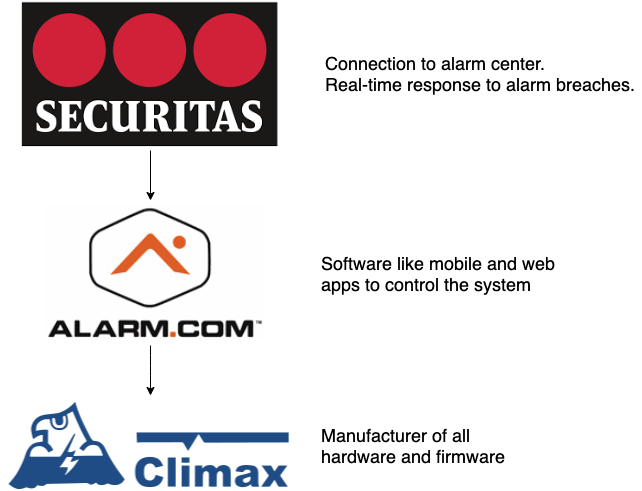
\includegraphics[width=0.7\textwidth]{images/company-structure.png}
    \caption{The companies behind the system.}
    \label{fig:company-structure}
\end{figure}

\section{Components and Software} \label{ch:system:components}
This section describes all the components and software of the system. Initially, all hardware components are described and their functionality. Lastly, all software components of the system are described. Note that the system supports many additional hardware components. The ones outlined below are only the ones part of the starter-kit.

\subsection{Hardware components} \label{ch:system:hardware}
The SecuritasHome starter-kit contains five hardware components, see figure \ref{fig:hardware-components}. These are described below. Note that the system supports many additional components, like smart locks for example. However, only the components included in the starter-kit are covered in this thesis.
\begin{figure}[!ht]
    \centering
    \begin{subfigure}[t]{0.33\textwidth}
        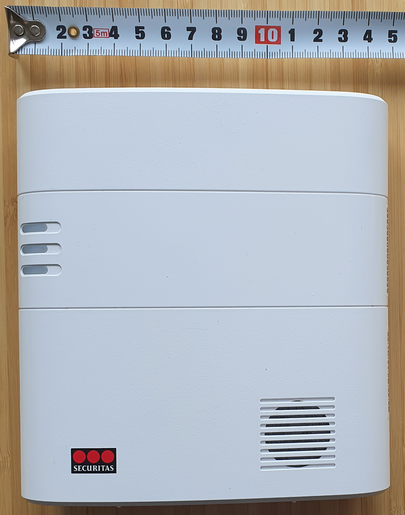
\includegraphics[height=2.15in]{images/main-panel.png}
        \caption{Main Panel}
        \label{fig:main-panel}
    \end{subfigure}%
    ~
    \begin{subfigure}[t]{0.33\textwidth}
        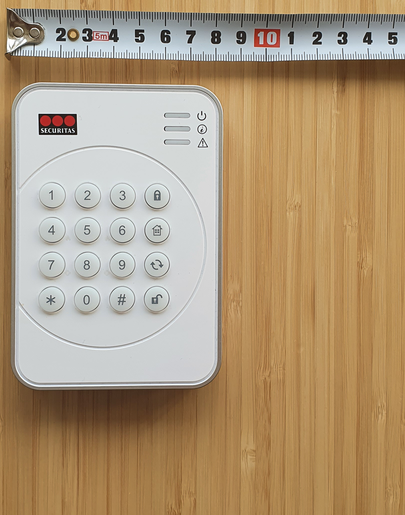
\includegraphics[height=2.15in]{images/keypad.png}
        \caption{Remote Keypad}
        \label{fig:remote-keypad}
    \end{subfigure}%
    ~
    \begin{subfigure}[t]{0.33\textwidth}
        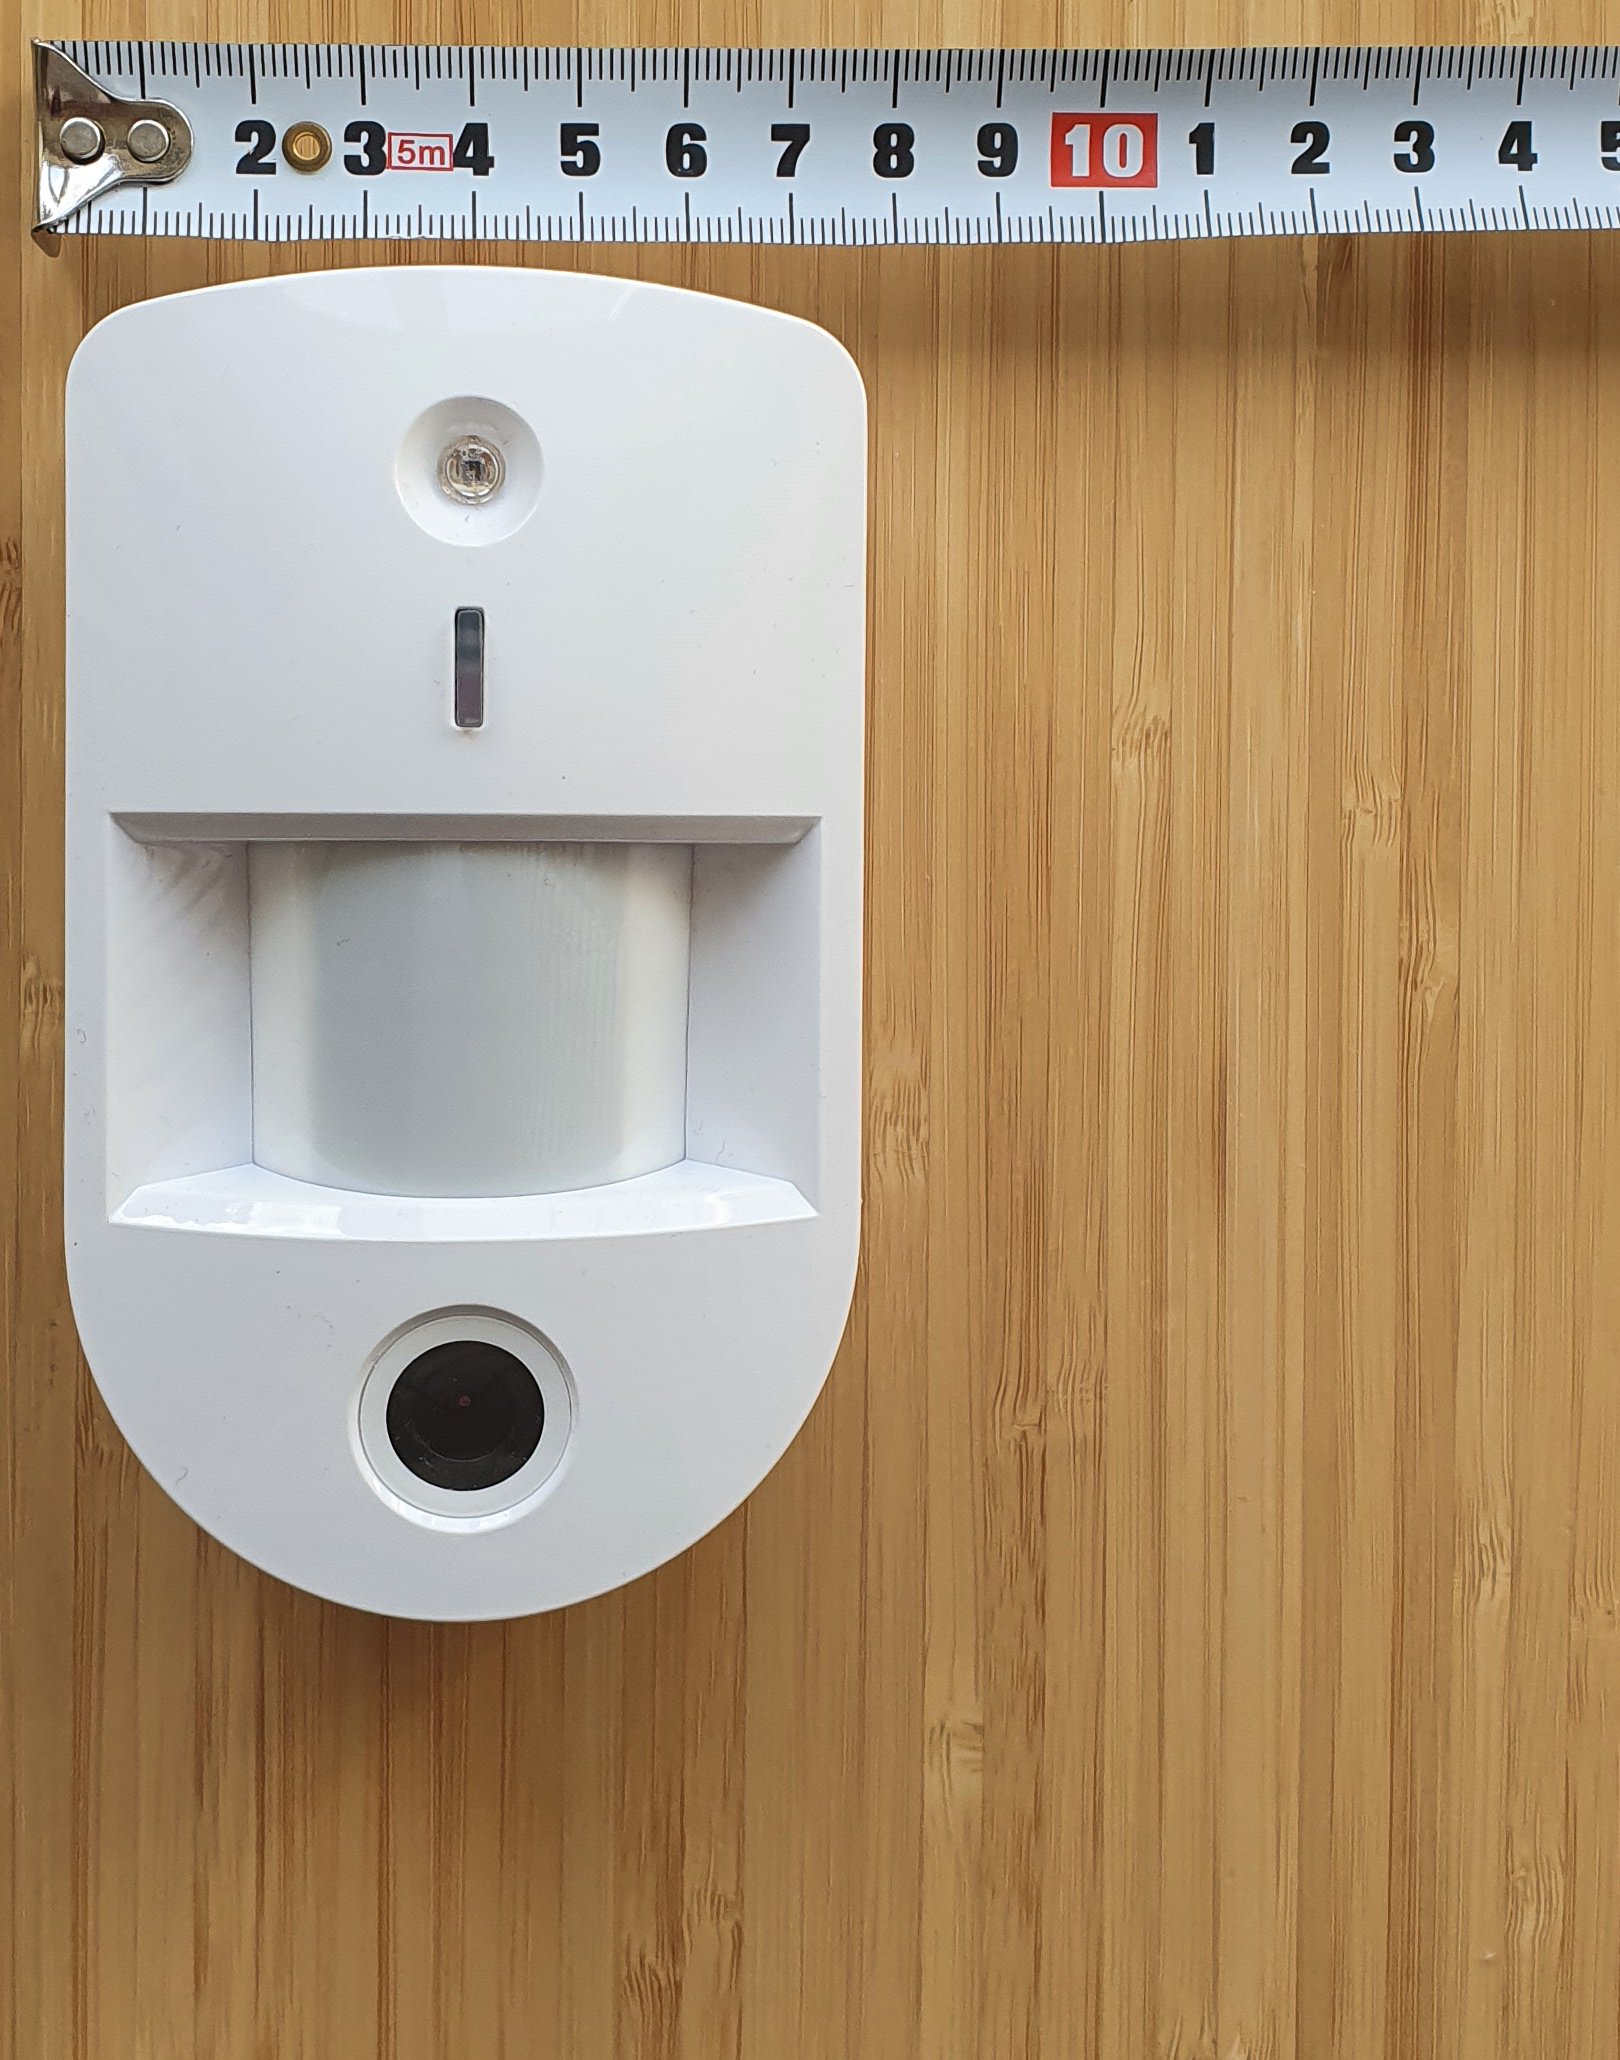
\includegraphics[height=2.15in]{images/camera.png}
        \caption{Motion Detection Camera}
        \label{fig:motion-camera}
    \end{subfigure}
    
    \begin{subfigure}[t]{0.33\textwidth}
        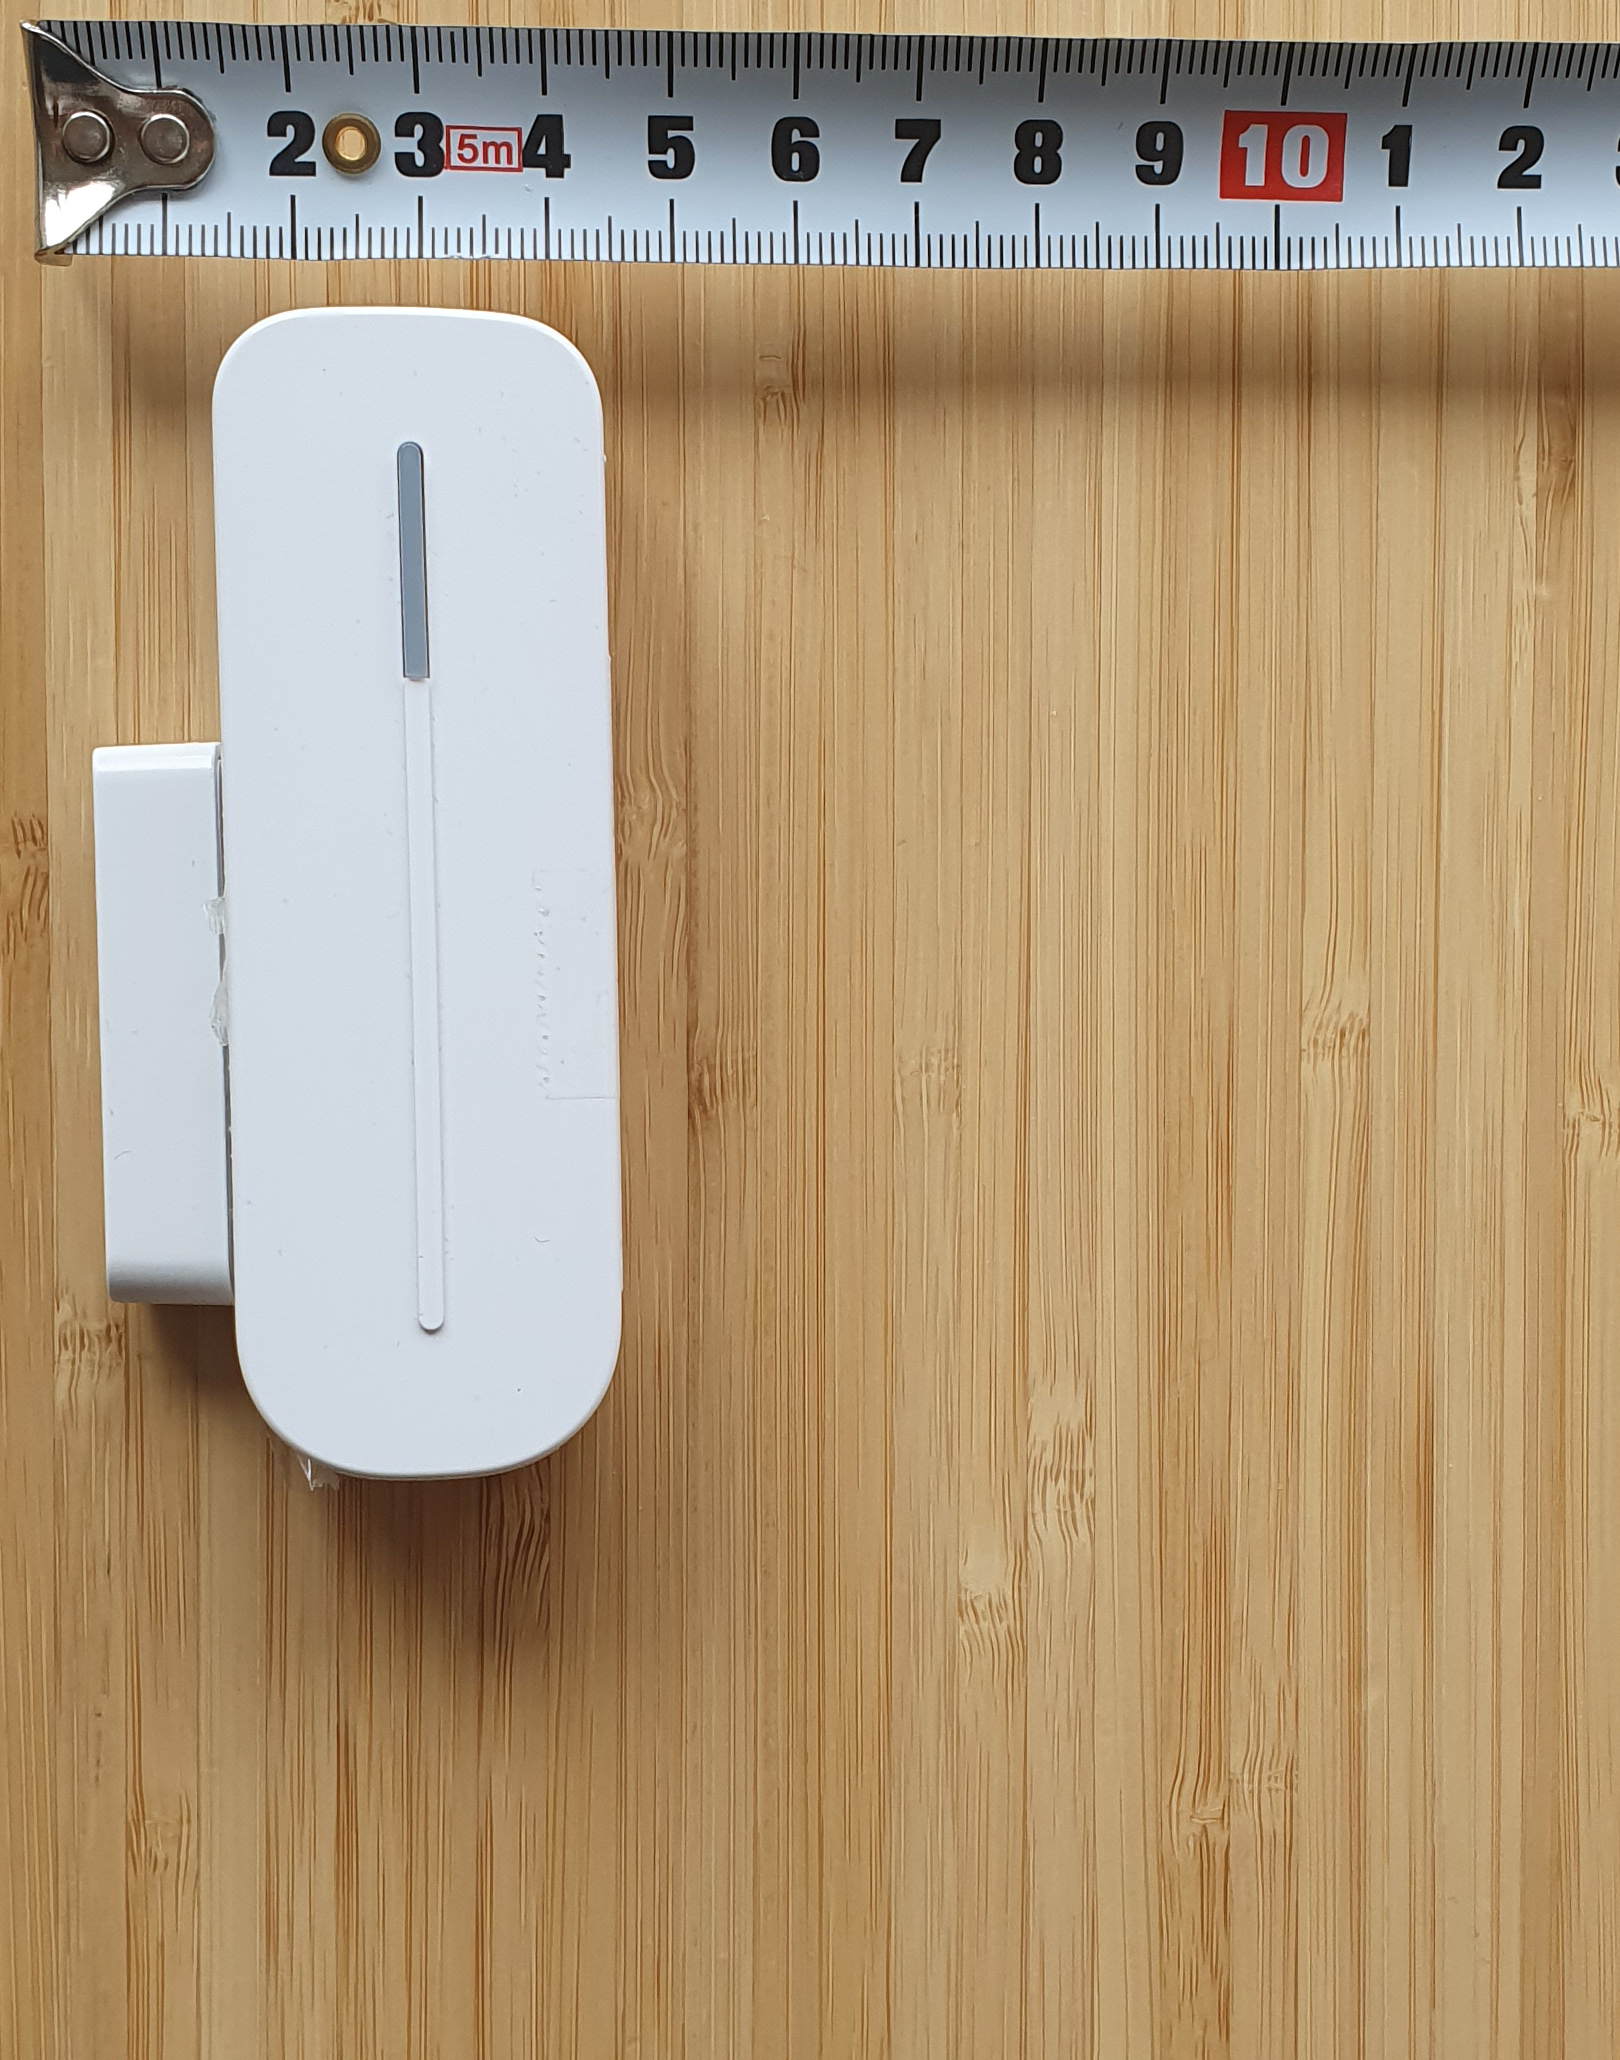
\includegraphics[height=2.15in]{images/door-contact.png}
        \caption{Door Contact Sensor}
        \label{fig:door-contact}
    \end{subfigure}%
    ~
    \begin{subfigure}[t]{0.33\textwidth}
        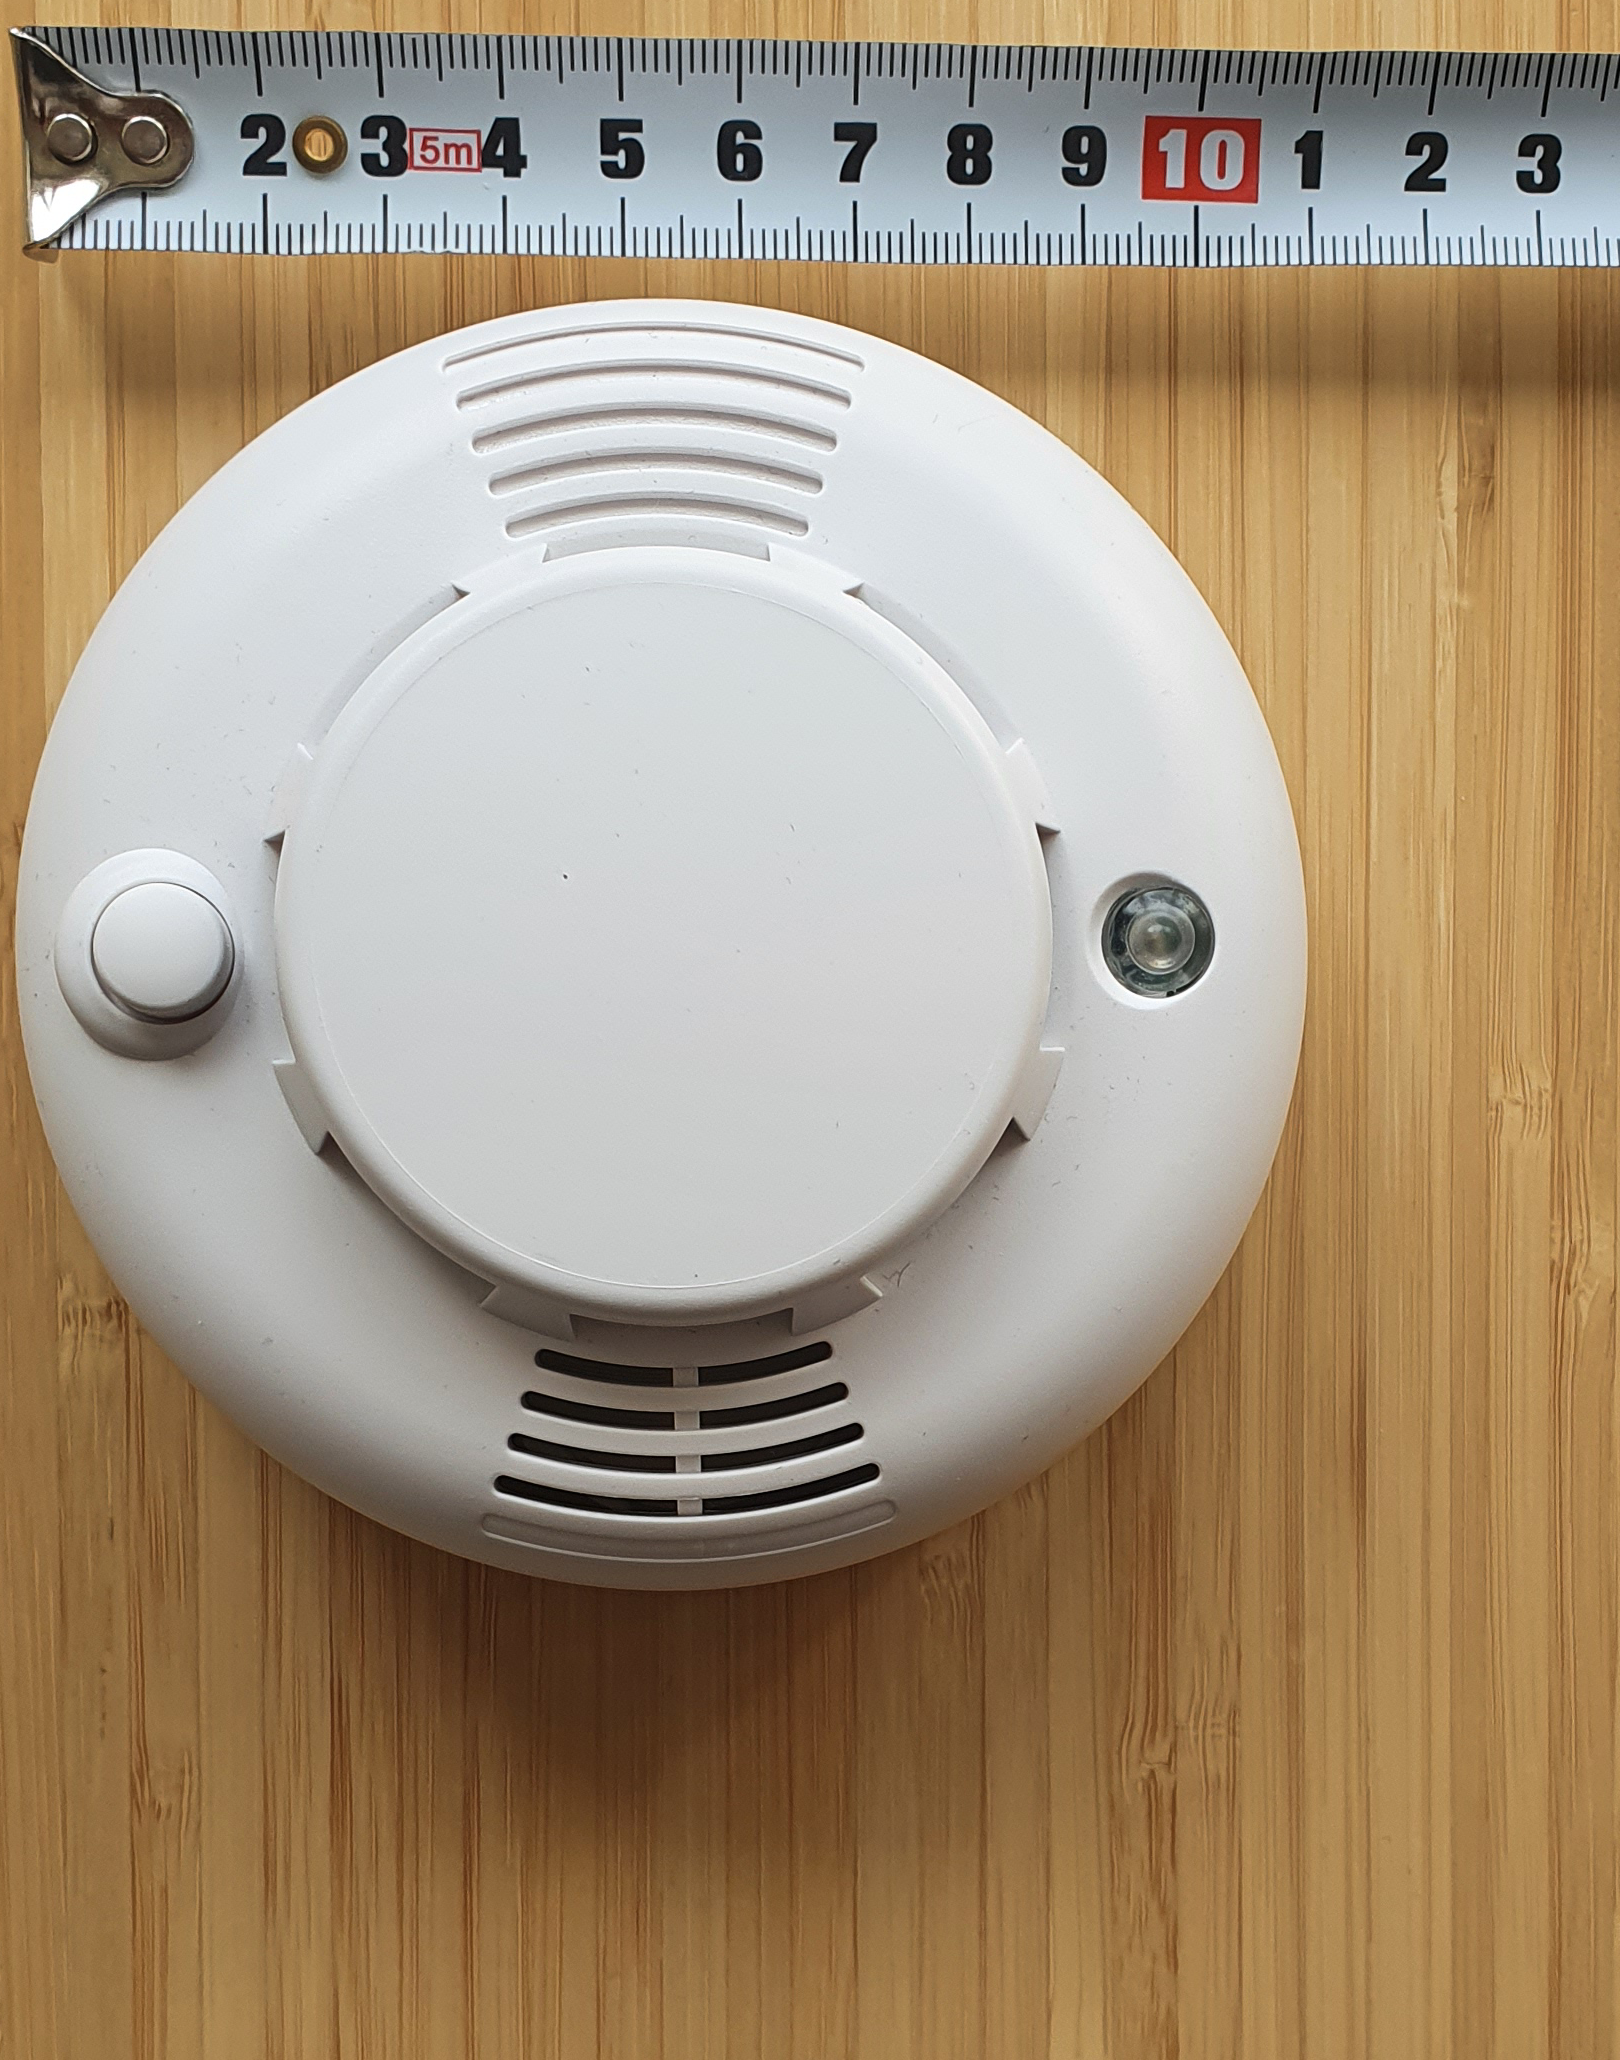
\includegraphics[height=2.15in]{images/smoke-detector.png}
        \caption{Smoke Detector}
        \label{fig:smoke-detector}
    \end{subfigure}
    \caption{The hardware components of the system}
    \label{fig:hardware-components}
\end{figure}
\subsubsection{Main Panel}
\textbf{Model number:} HSGW-G8-3G/LTE-ZW-F1 433/868 \\
\textbf{FCCID:} GX9HSGWF1919 \\
The main panel, see figure \ref{fig:main-panel}, is the \textit{"brains"} of the system so to speak. It handles communication with all other hardware devices as well as external servers. Through radio wave communication it talks to the other hardware peripherals of the system. It uses 3G telecommunication to talk to the external servers.

\subsubsection{Remote Keypad}
\textbf{Model number:} KPT-23-EL-F1 \\ % could also be KPT-23N-EL-F1, not sure
\textbf{FCCID:} GX9KPF1 \\ % This says KPF but it looks the same..
The remote keypad is a 16 button keypad used to arm and disarm the system using a personal 4 digit pin. See figure \ref{fig:remote-keypad}. This device talks to the main panel over radiowave communication.

\subsubsection{Motion Detection Camera}
\textbf{Model number:} VST-862-F1 \\
\textbf{FCCID:} GX9862 \\
This device, see figure \ref{fig:motion-camera}, features an infra-red sensor to detect motion, and a camera to survey the location. When triggered the device takes two pictures which are sent to the main panel. It is not a surveillance camera, meaning it does not continuously take pictures. The camera is only active when motion is detected and the alarm is triggered, presumably to save power.

\subsubsection{Door Contact Sensor}
\textbf{Model number:} DC-23-F1 \\
\textbf{FCCID:} GX9DC23 \\
This device, see figure \ref{fig:door-contact}, senses when a door or window is opened. A small external magnet is placed on the door/window close to the device. When these are separated the device is triggered and communicates with the main panel over radio wave communication.

\subsubsection{Smoke Detector}
\textbf{Model number:} SD-8EL \\
\textbf{FCCID:} GX9SD8ELF1919 \\
This device is a smoke detector, see figure \ref{fig:smoke-detector}. It communicated with the main panel over radio-waves and also includes a siren which triggers when it detects smoke.

\subsection{Software} \label{ch:system:software}
This section details the three software entry points from where the user can control the alarm and view it's state.

\subsubsection{Web portal}
The web portal is a webpage created by the American company \textit{Alarm.com}, see figure \ref{fig:company-structure}, hosted at \url{https://www.alarm.com/web/system/}. From the landing page, see figure \ref{fig:web-landing-page}, the user can see the following:
\begin{itemize}
    \item If the system has any issues. This can be seen in the \textit{System OK} box in figure \ref{fig:web-landing-page}.
    \item The state of each sensor of the system, like the door contact sensor (see figure \ref{fig:door-contact}).
    \item The arm/disarm state of the system.
    \item The latest photograph taken by the motion detection camera (see figure \ref{fig:motion-camera}).
\end{itemize}
Crucially, from the landing page, the user can also easily arm or disarm the system, see figure \ref{fig:web-arming}. Beyond this, the user can also see a list of recent activity in the system, change users personal four digit pin codes, and create new users.

\begin{figure}[!ht]
    \centering
    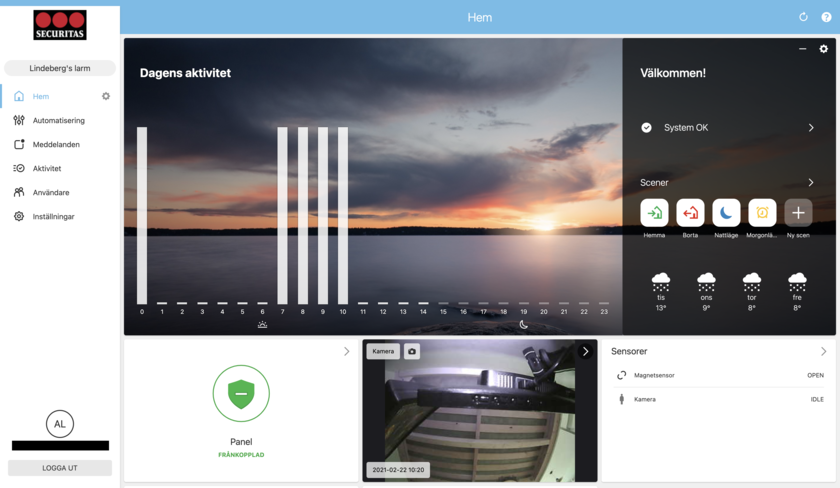
\includegraphics[width=\textwidth]{images/landing-page-web.png}
    \caption{The web portal landing page.}
    \label{fig:web-landing-page}
\end{figure}
\begin{figure}[!ht]
    \centering
    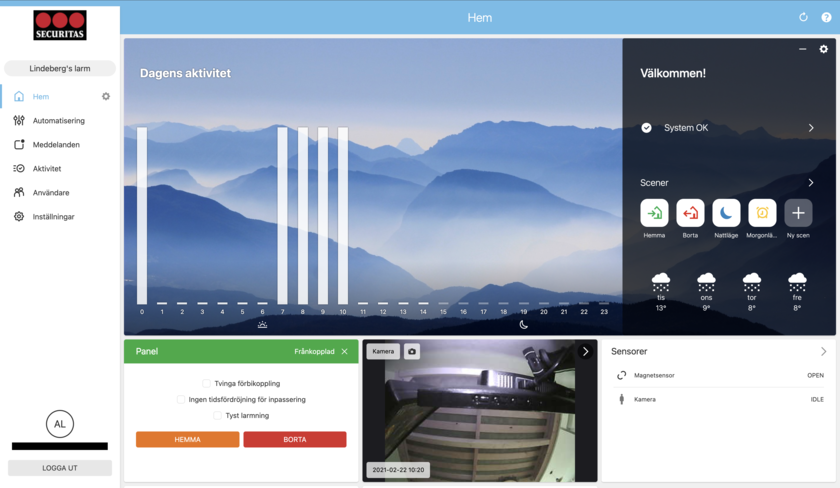
\includegraphics[width=\textwidth]{images/arming-web.png}
    \caption{Arming the alarm from the web portal.}
    \label{fig:web-arming}
\end{figure}

\subsubsection{Mobile application}
The system can also be controlled and administrated via a mobile application, free to download via the \textit{Google Play Store}, called \textit{Securitas Connect}\footnotelink{https://play.google.com/store/apps/details?id=com.alarm.alarmmobile.android.securitas}{2021-03-30}. As explained previously, while the application is branded by Securitas, it is created and developed by \textit{Alarm.com}. The interface very closely resembles the web portal, see figure \ref{fig:mobile-landing-page}, and offers identical functionality, see figure \ref{fig:mobile-landing-page}.
\begin{figure}[!ht]
    \centering
    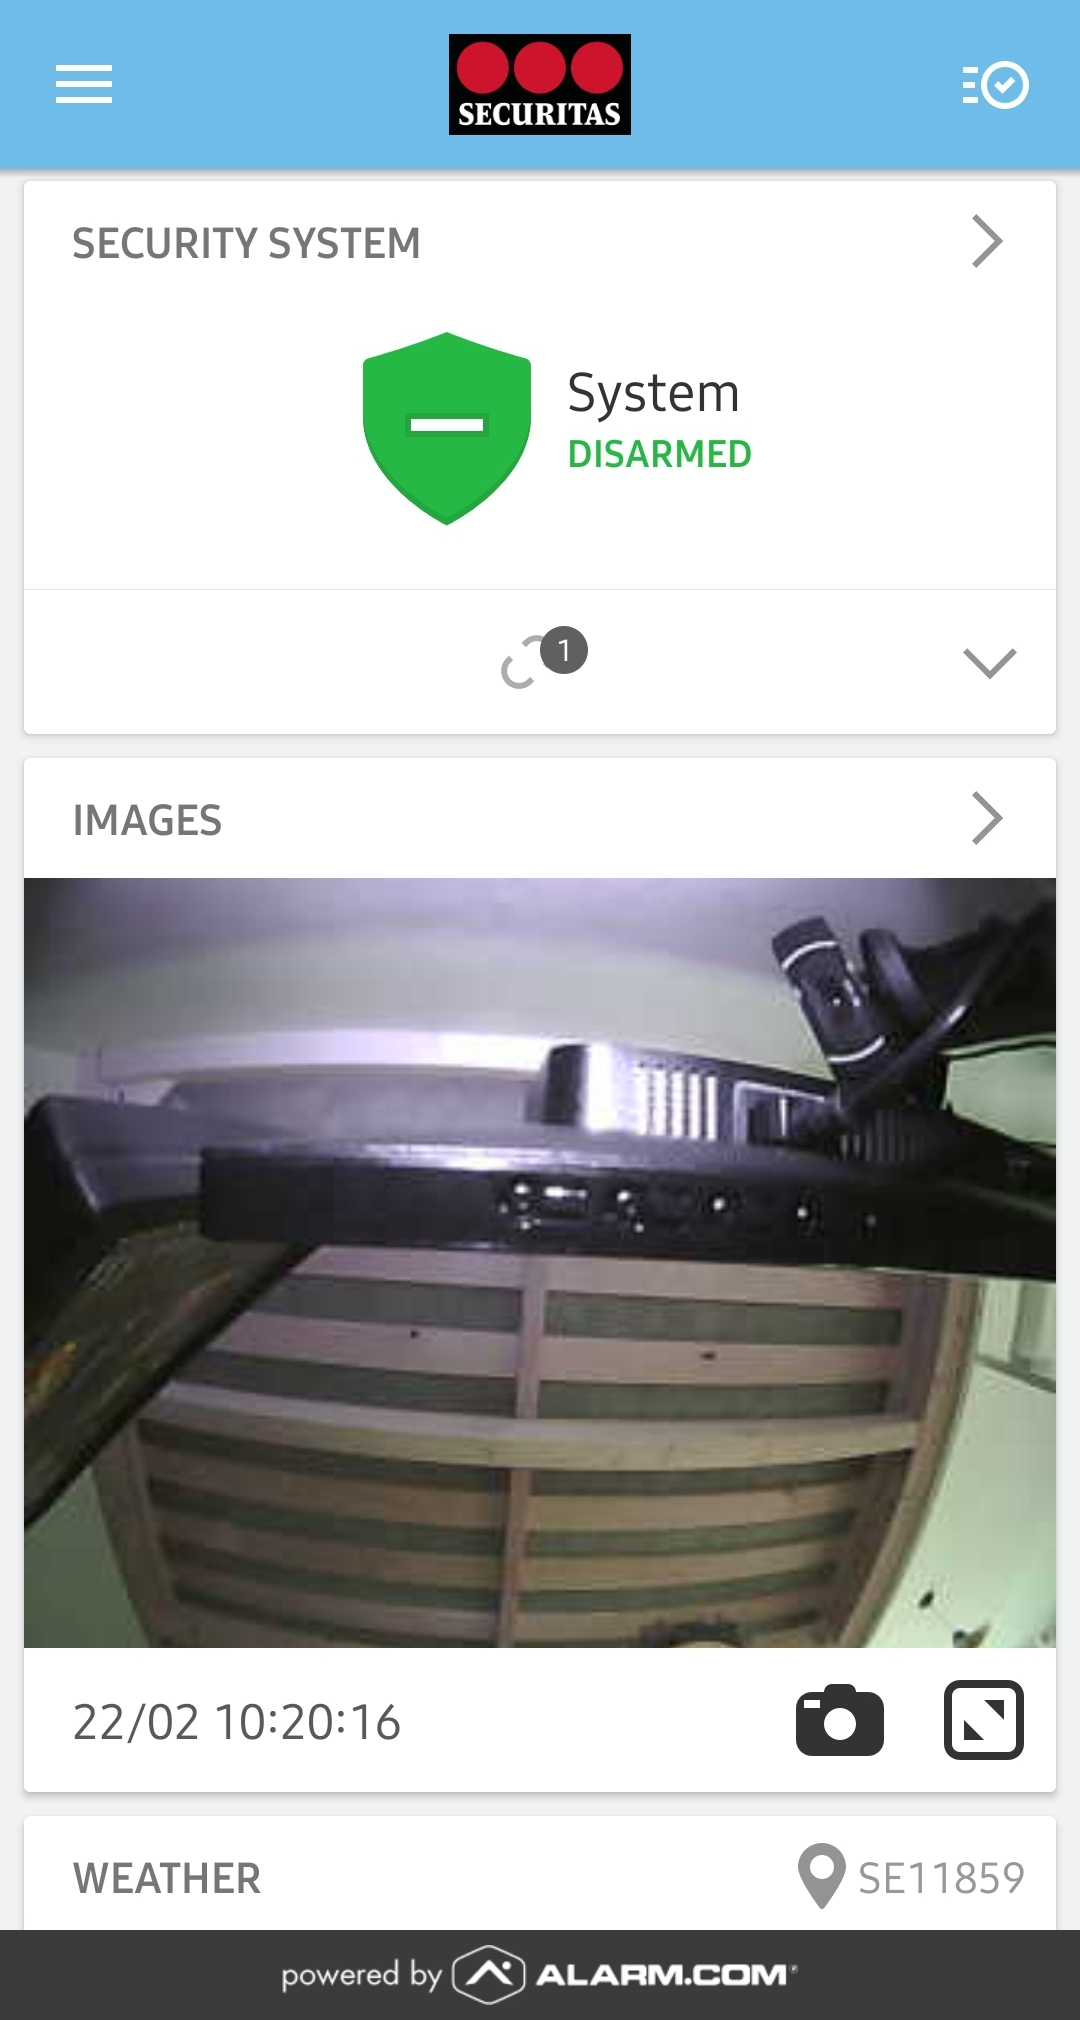
\includegraphics[width=0.5\textwidth]{images/mobile-landing-page.jpg}
    \caption{The android mobile app landing page.}
    \label{fig:mobile-landing-page}
\end{figure}

\subsubsection{Local web admin page}
Beyond the two applications created by \textit{Alarm.com} described above, the main panel (see figure \ref{fig:main-panel}) hosts a web server on the local network. This feature is undocumented, and is presumably not meant to be used or found by the regular, non-tech-savvy consumer. The page is not hosted on any domain name, as far as the author is aware, and instead has to be accessed directly via the main panels local IP address on port 80. The landing page of this web server, see figure \ref{fig:local-landing-page}, is quite simple and shows some basic information about the system such as the MAC address, IMEI number of the cellular communication, etc. Beyond that, the site only has two actions the user can do. One is to perform a "\textit{Phone Test}", to presumably test the connection to the mobile 3G network, and the other is a "\textit{Network Scan}". Once the network scan has completed, the page shows a list of all reachable telecommunication towers, see figure \ref{fig:local-network-scan}.
\begin{figure}[!ht]
    \centering
    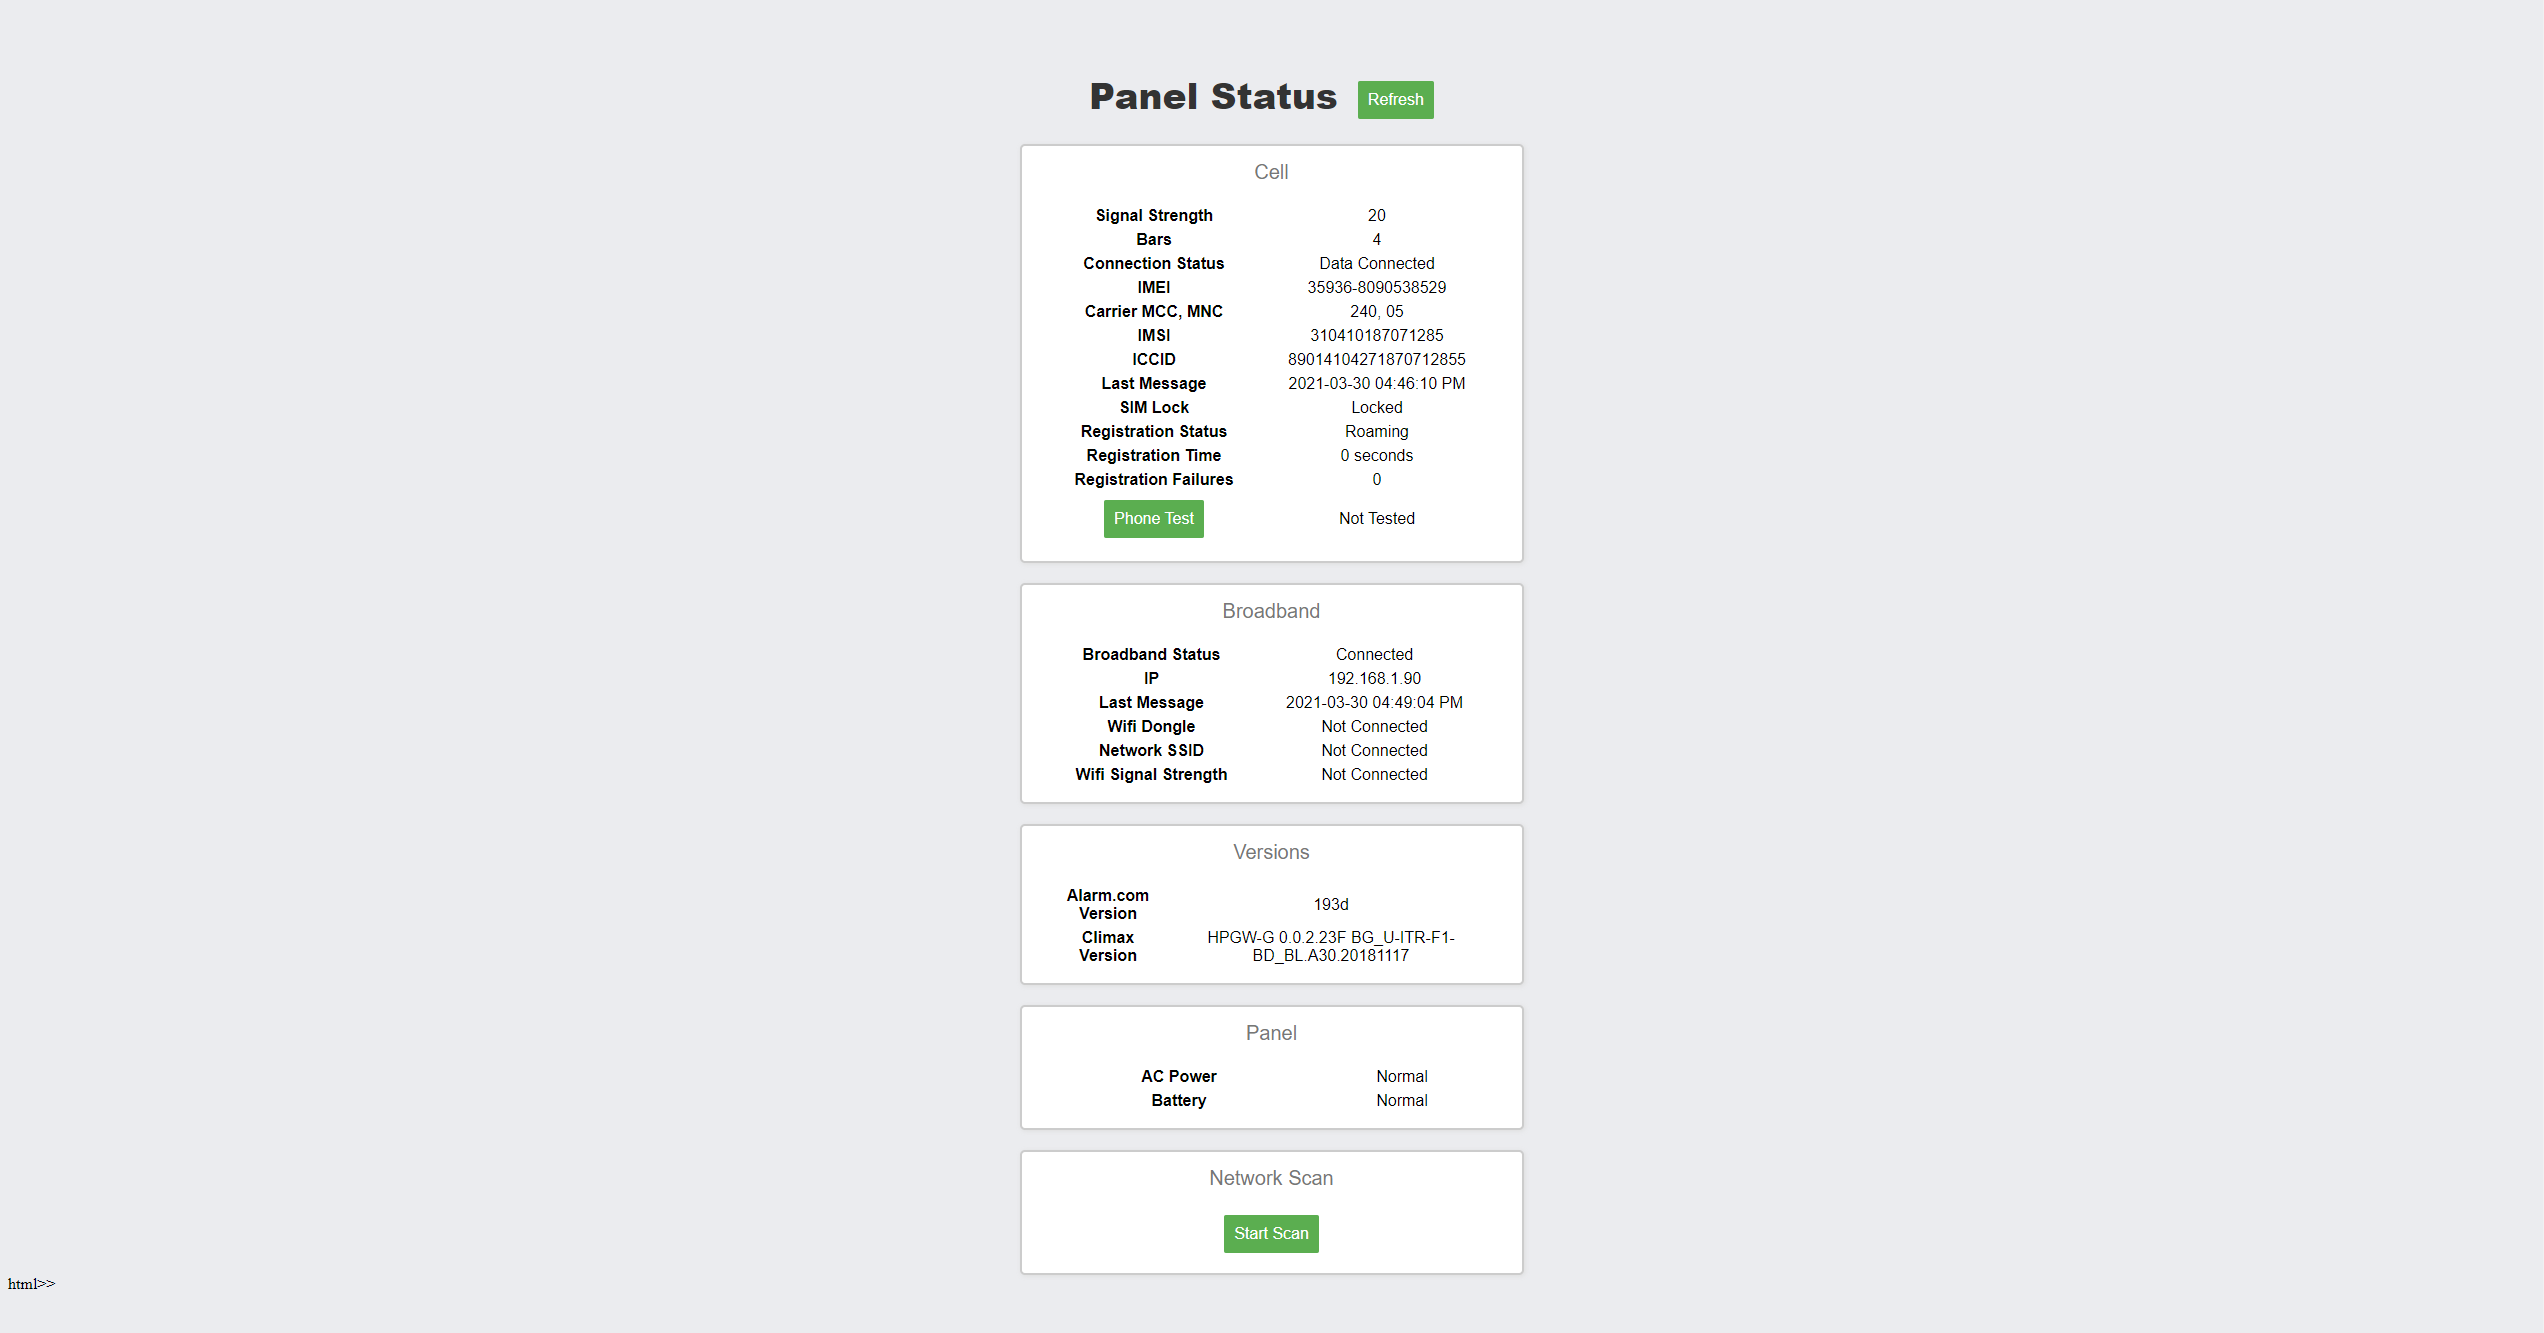
\includegraphics[width=\textwidth]{images/local-landing-page.png}
    \caption{The local web server's landing page.}
    \label{fig:local-landing-page}
\end{figure}
\begin{figure}[!ht]
    \centering
    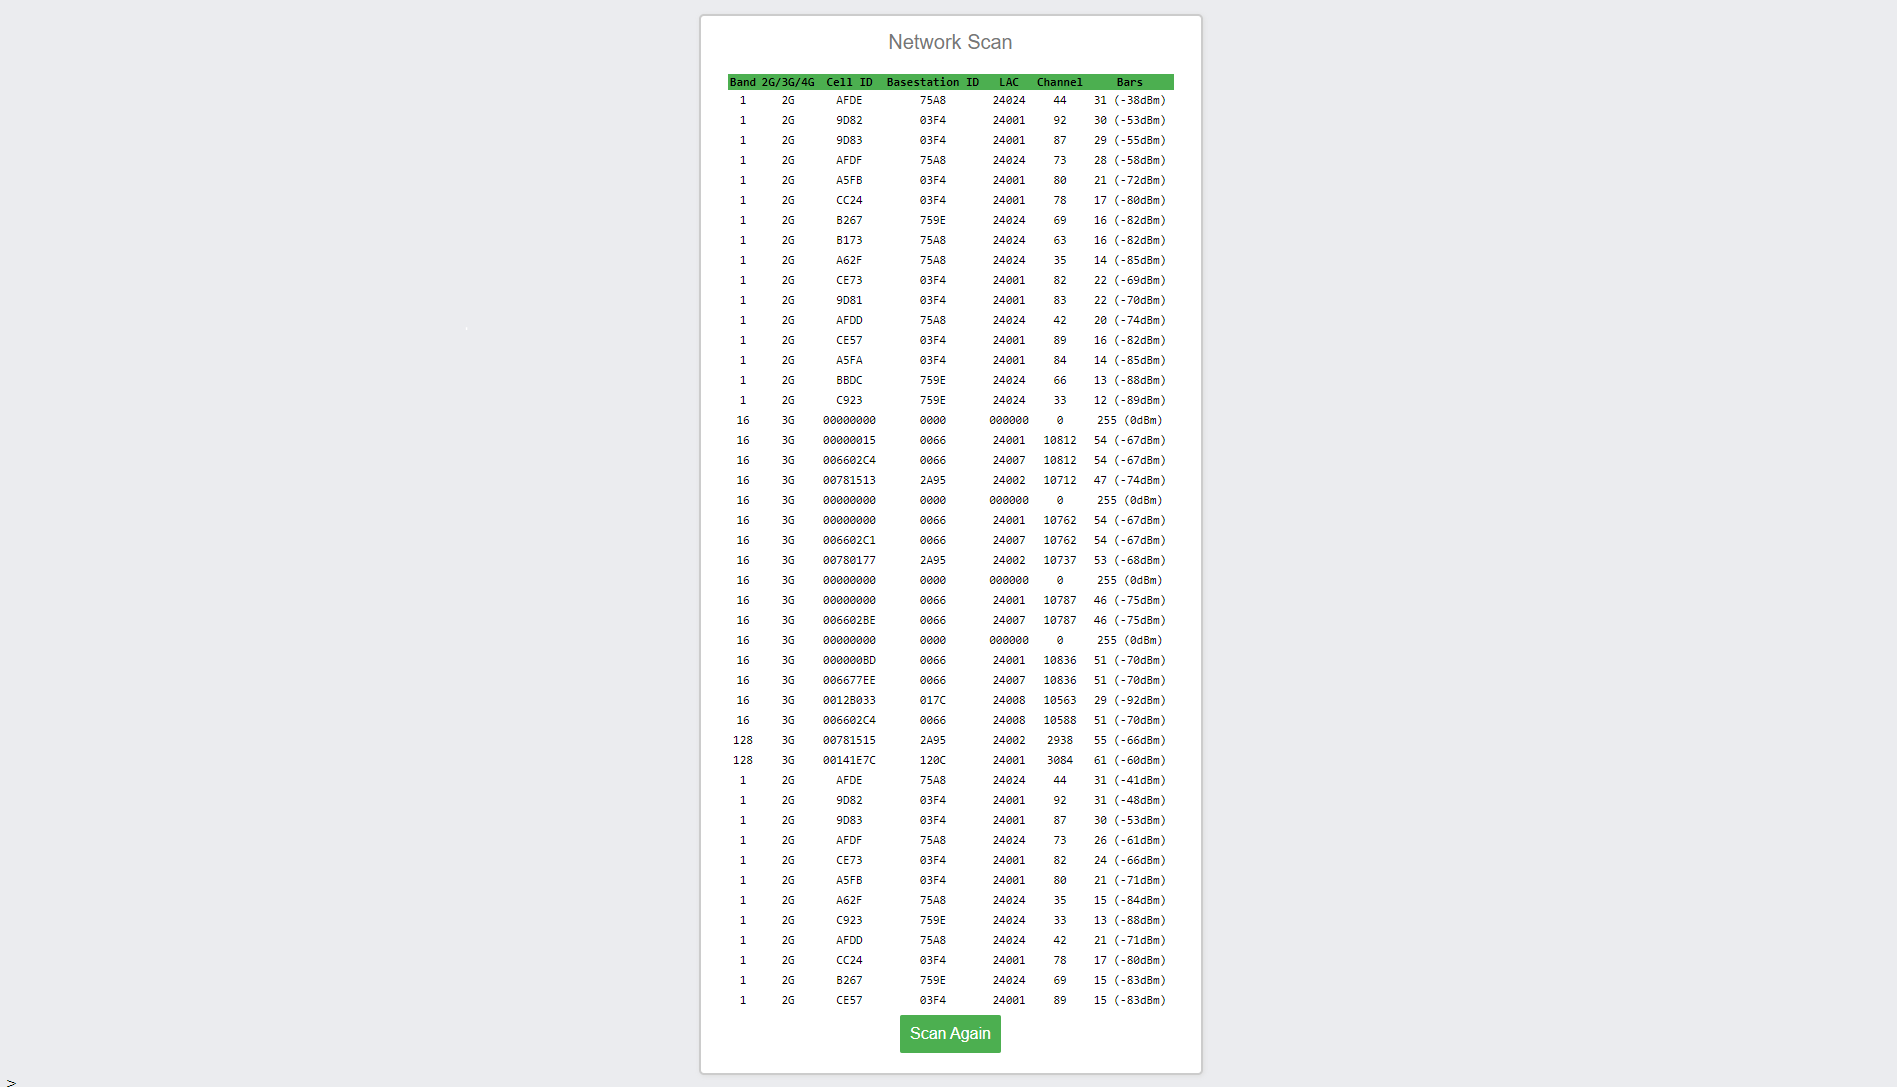
\includegraphics[width=\textwidth]{images/local-network-scan.png}
    \caption{A mobile network scan from the local web server.}
    \label{fig:local-network-scan}
\end{figure}
\begin{figure}[!ht]
    \centering
    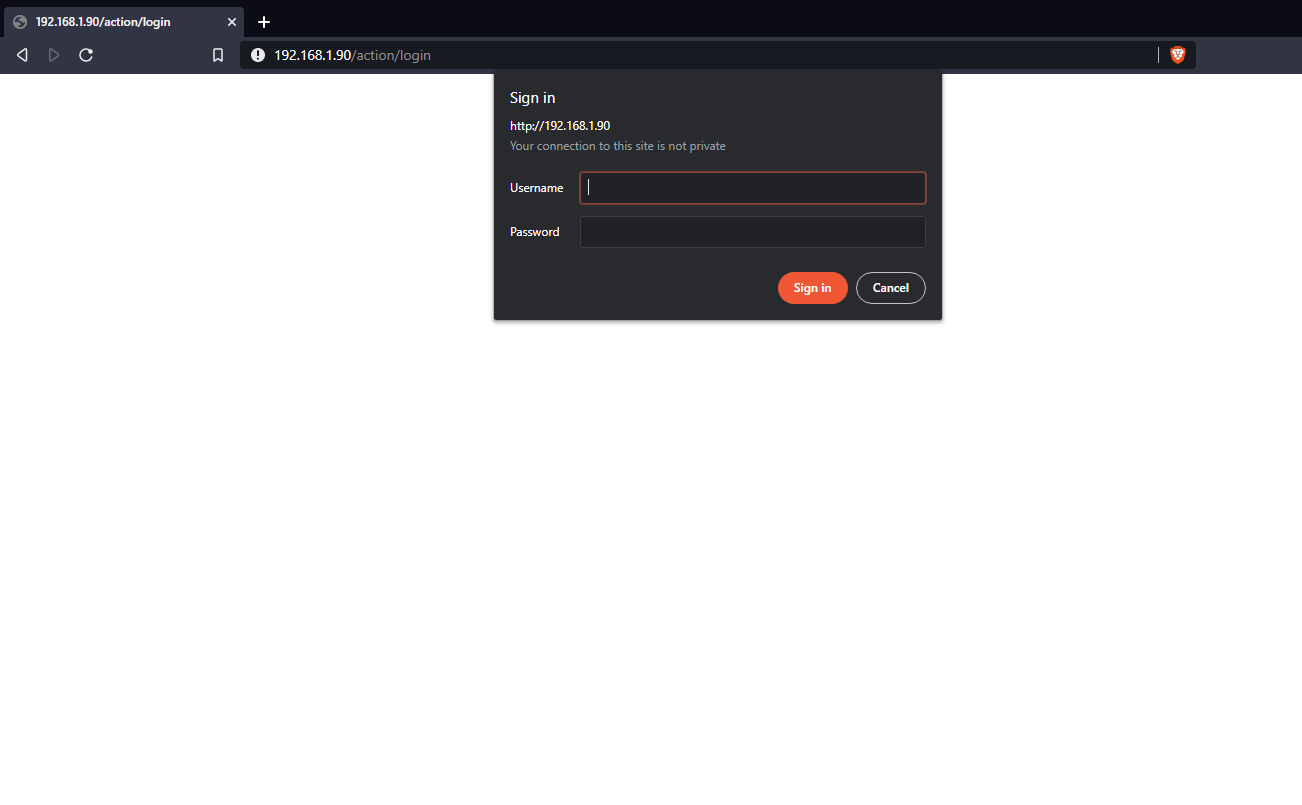
\includegraphics[width=\textwidth]{images/local-login-page.png}
    \caption{The local web server's HTTP Basic Auth login page.}
    \label{fig:local-login-page}
\end{figure}
\begin{figure}[!ht]
    \centering
    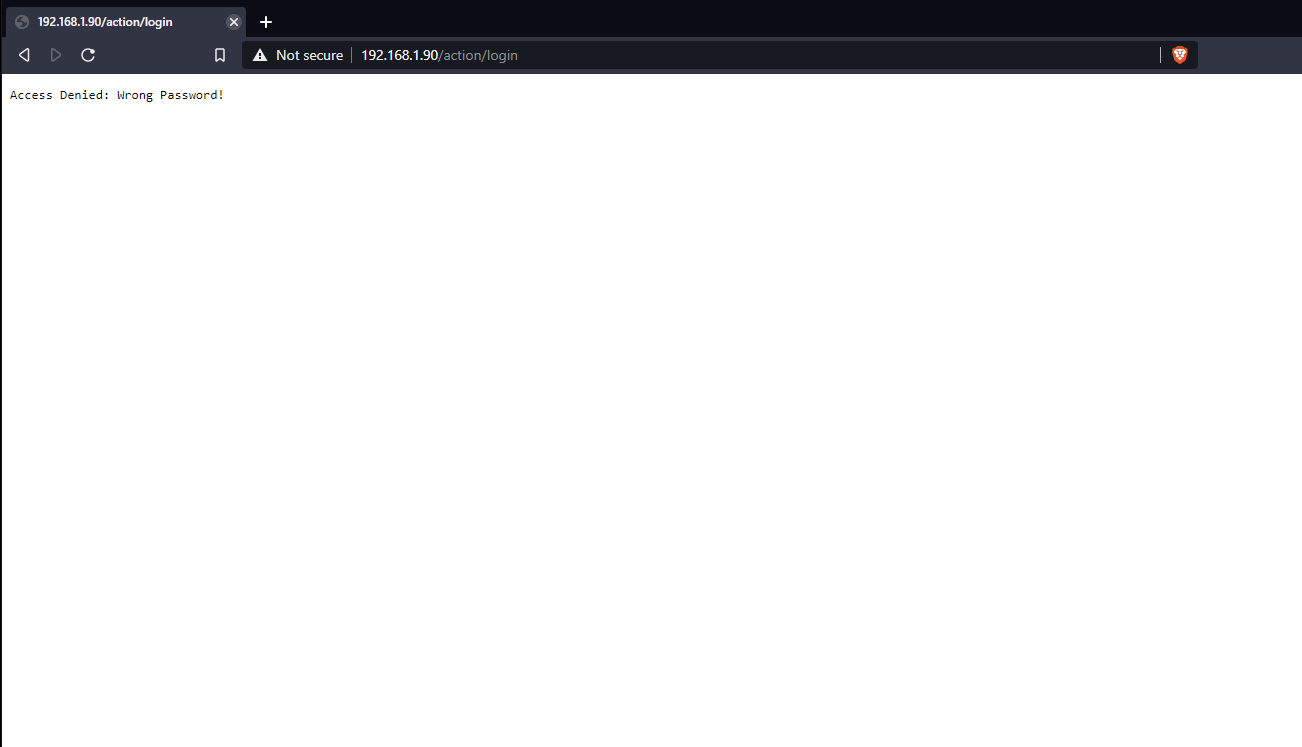
\includegraphics[width=\textwidth]{images/local-login-denied.png}
    \caption{A failed login attempt on the local web server.}
    \label{fig:local-login-denied}
\end{figure}
Additionally, the web page features an undocumented login page on the path \texttt{/action/login}, see figure \ref{fig:local-login-page}. This page lets the user authenticate using \textit{HTTP Basic auth}. The credentials here are not tied to the users account on the aforementioned web portal or mobile applications. Presumably this is purely meant as a backdoor for \textit{Climax Technology} for debugging purposes, and not meant to be used by the user of the system. If wrong credentials are entered the user is presented with a static message, saying they have the wrong password (see figure \ref{fig:local-login-denied}), providing zero additional functionality.
\chapter{Threat Model} \label{ch:threat-model}
This chapter contains the threat model established for the system under scrutiny, which was used to identify and document all threats to the system. The methodology and threat model technique is described in section \ref{ch:method:threat-modeling}.

\section{Identified Assets}
As part of the first phase of our threat modeling technique, assets of the system were identified. These can be found in table \ref{tb:assets}.
\begin{table}[!ht]
    \centering
    \begin{tabularx}{\textwidth}{r X}
        \hline
        \textbf{ID} & \textbf{Description}
        \\ \hline
        1  & Physical access to the house
        \\
        2  & Personal four digit pin
        \\
        3  & Arm/disarm state of the system
        \\
        4  & Door contact sensor state
        \\
        5  & Authentication to the admin web application
        \\
        6  & Triggered alarm state
        \\
        7  & Perhaps more?
        \\ \hline
    \end{tabularx}
    \caption{The identified assets of the system}
    \label{tb:assets}
\end{table}

\section{Architecture Overview}
This section contains an architecture overview of the system. Included in this are three components presented below. First is a list of all identified use cases of the system. Second, is a diagram visually presenting all components of the system, how they interact, and the data flow of the system. Lastly, a table of all identified technologies used in the system are presented.

\subsection{Use cases}
As part of the architecture overview, all use cases of the system were identified. These are the use cases a regular user would encounter when using the system normally. The use cases are documented in table \ref{tb:use-cases}.
\begin{table}[!ht]
    \centering
    \begin{tabularx}{\textwidth}{r X}
        \hline
        \textbf{ID} & \textbf{Description}
        \\ \hline
        1  & The user arms/disarms the system via the remote keypad panel
        \\
        2  & The user arms/disarms the system via the web portal
        \\
        3  & The user arms/disarms the system via the mobile app
        \\
        4  & The user receives a notification about a state change in the system
        \\
        5  & Perhaps more?
        \\ \hline
    \end{tabularx}
    \caption{Use cases of the system}
    \label{tb:use-cases}
\end{table}

\begin{figure}[!ht]
    \centering
    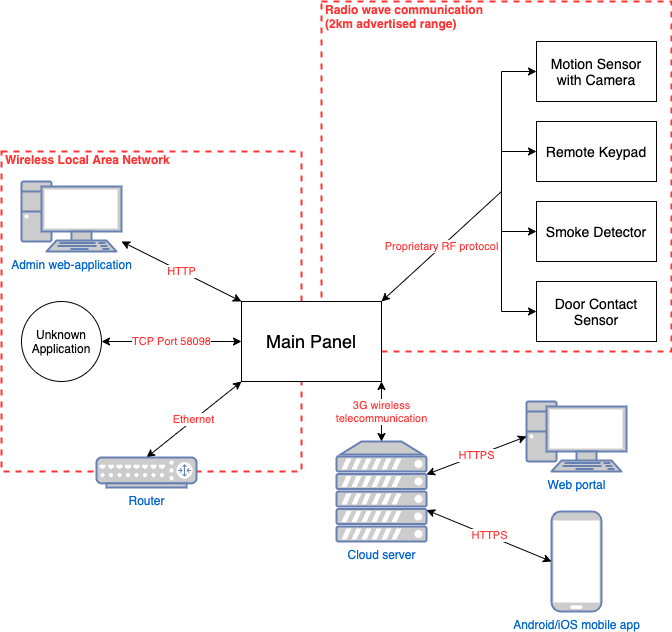
\includegraphics[width=\textwidth]{images/system-overview.png}
    \caption{Data flow diagram of the system}
    \label{fig:system-overview}
\end{figure}

\subsection{System Technologies}
Table \ref{tb:system-technologies} contains all identified technologies present in the system. There are undoubtedly additional technologies used but these are the ones identified and relevant.
\begin{table}[!ht]
    \centering
    \begin{tabularx}{\textwidth}{l X}
        \hline
        \textbf{Technology}  & \textbf{Description}
        \\ \hline
        Main Panel & Linux 2.6-2.30. Hosts a web server over HTTP, using Mongoose (an embedded web server), version unknown. Unknown application listening on TCP port 58098. Hosts DNS on TCP/UDP port 53. Has a USB and ethernet port.
        \\ \hline
        HTTP  & Protocol used by the admin web application. A clear text protocol, used to communicate with the web admin panel.
        \\ \hline
        F1 RF protocol  & A proprietary \gls{RF} protocol from the hardware manufacturer, Climax Technology. Uses 868 MHz frequency. This is an undocumented protocol, meaning no technical specification have been publicized.
        \\ \hline
        Mongoose web server  & An open source web server, in C. Used by the main panel to host the local admin web page, version unknown.
        \\ \hline
    \end{tabularx}
    \caption{Technologies used in the system}
    \label{tb:system-technologies}
\end{table}

\section{Decomposition of the system}
This section presents the results of the fourth step of the threat modeling technique. Lastly, all identified entry points of the system are listed.

\subsection{Entry points}
As part of the decomposition of the system, all entry points of the system was identified. These are essentially all points of contact an attacker could probe. The entry points are documented in table \ref{tb:entry-points}.
\begin{table}[!ht]
    \centering
    \begin{tabularx}{\textwidth}{l X}
        \hline
        \textbf{Entry point} & \textbf{Description}
        \\ \hline
        Local web admin page  & See section \ref{ch:system:software}. Provides very basic functionality but no control over the system. Has an undocumented login page via \textit{HTTP Basic Auth}. Data is transferred over HTTP on the local network.
        \\ \hline
        Unknown application  & This is a completely undocumented process, listening on TCP port 58098. Closes the connection when sent data. Becomes unresponsive when sent certain data like \texttt{[]} and \texttt{\{\}} (presumably it crashes).
        \\ \hline
        Main panel  & The physical device features an Ethernet port to connect to the local network, as well as a USB port for unknown purposes. It communicates with other devices over a 868 GHz proprietary \gls{RF} protocol.
        \\ \hline
        3G telecommunication  & The device has a SIM-card and communicates over the 3G telecommunication network.
        \\ \hline
        \gls{RF} communication  & The device talks to the other peripherals over a proprietary \gls{RF} protocol, called \textit{F1}\footnotelink{https://www.climax.com.tw/new/f1-features-new.php}{2021-04-02}. There seems to be little to no information available to the public about this protocol, other than it's operating frequency of 868 GHz.
        \\ \hline
        USB port  & The device has a USB 2.0 Type-A connector.
        \\ \hline
        Firmware  & The firmware of the system.
        \\ \hline
    \end{tabularx}
    \caption{The entry points of the main panel}
    \label{tb:entry-points}
\end{table}

\section{Identified Threats} \label{ch:threat-model:threats}
The following section contains all identified threats. These are categorized after the threat categories of the STRIDE model. For an explanation of the model and a description of each category see section \ref{ch:method:stride}.

\subsection{Spoofing Identity}
\begin{itemize}
    \item Spoof the remote keypad.
    \item Spoof the door contact sensor.
    \item Spoof the smoke detector.
    \item Spoof the motion detection camera.
    \item Spoof the remote keypad.
\end{itemize}

\subsection{Tampering with data}
\begin{itemize}
    \item [TODO]
\end{itemize}

\subsection{Repudiation}
\begin{itemize}
    \item [TODO]
\end{itemize}

\subsection{Information Disclosure}
\begin{itemize}
    \item [TODO]
\end{itemize}

\subsection{Denial of Service}
\begin{itemize}
    \item [TODO]
\end{itemize}

\subsection{Elevation of privilege}
\begin{itemize}
    \item [TODO]
\end{itemize}

\chapter{Penetration testing} \label{ch:pentesting}
This chapter details all penetration tests that were performed on the system. These were derived from the threat model created in chapter \ref{ch:threat-model}. All penetration tests are described in the format outlined below. If an aspect of the test was considered simple then one or more parts have been omitted.
\begin{itemize}
    \item \textit{Introduction}. Describes the attack vector that this penetration test will explore.
    \item \textit{Background}. Details the required background knowledge to perform and evaluate this penetration test, if any.
    \item \textit{Method}. Describes in detail how the test was performed, e.g in what environment, with what tools, what commands were used, etc.
    \item \textit{Results}. Describes the findings of the penetration test.
    \item \textit{Discussion}. This section contains a discussion about the reliability, validity, and generalizability of the results.
\end{itemize}

\section{Task 1: Online Password Attack}
An online password attack refers to probing an active login, as opposed to an offline attack where you for example might try to crack a hash of a leaked database. This attack involves using some type of approach to test many passwords of a login form to try and find valid credentials.

\subsection{Background}
\subsection{Method}
\subsection{Results}
\subsection{Discussion}
\chapter{Discussion}\todo[inline]{This can be a separate chapter or a section
  in the previous chapter.}
\todo[inline, backgroundcolor=aqua]{Diskussion}
\label{ch:discussion}
\begin{swedishnotes}
Förbättringsförslag?
\end{swedishnotes}

\cleardoublepage
\chapter{Conclusions and Future work}
\todo[inline, backgroundcolor=aqua]{Slutsats och framtida arbete}
\label{ch:conclusionsAndFutureWork}
Add text to introduce the subsections of this chapter.

\section{Conclusions}
\todo[inline]{Describe the conclusions (reflect on the whole introduction given in Chapter 1).}
\todo[inline, backgroundcolor=aqua]{Slutsatser}
\label{sec:conclusions}
  
Discuss the positive effects and the drawbacks.\\
Describe the evaluation of the results of the degree project.\\
Did you meet your goals?\\
What insights have you gained?\\
What suggestions can you give to others working in this area?\\
If you had it to do again, what would you have done differently?\\

\begin{swedishnotes}
Träffade du dina mål?
Vilka insikter har du fått?
Vilka förslag kan du ge till andra som arbetar inom detta område?
Om du hade att göra igen, vad skulle du ha gjort annorlunda?
\end{swedishnotes}

\section{Limitations}
\todo[inline]{What did you find that limited your
  efforts? What are the limitations of your results?}
\todo[inline, backgroundcolor=aqua]{Begränsande faktorer}
\label{sec:limitations}
\begin{swedishnotes}
Vad gjorde du som begränsade dina ansträngningar? Vilka är begränsningarna i dina resultat?
\end{swedishnotes}

\section{Future work}
\todo[inline]{Describe valid future work that you or someone else could or should do.\\
Consider: What you have left undone? What are the next obvious things to be done? What hints can you give to the next person who is going to follow up on your work?
}
\todo[inline, backgroundcolor=aqua]{Vad du har kvar ogjort?\\
Vad är nästa självklara saker som ska göras?\\
Vad tips kan du ge till nästa person som kommer att följa upp på ditt arbete?
}
\label{sec:futureWork}

Due to the breadth of the problem, only some of the initial goals have been
met. In these section we will focus on some of the remaining issues that
should be addressed in future work. ...

\subsection{What has been left undone?}
\label{what-has-been-left-undone}

The prototype does not address the third requirment, i.e., a yearly
unavailability of less than 3 minutes, this remains an open problem. ...

\subsubsection{Cost analysis}

The current prototype works, but the performance from a cost perspective makes
this an impractical solution. Future work must reduce the cost of this
solution, to do so a cost analysis needs to first be done. ...

\subsubsection{Security}

A future research effort is needed to address the security holes that results
from using a self-signed certificate. Page filling text mass. Page filling
text mass. ...


\subsection{Next obvious things to be done}

In particular, the author of this thesis wishes to point out xxxxxx remains as
a problem to be solved. Solving this problem is the next thing that should be
done. ...

\section{Reflections}
\todo[inline]{What are the relevant economic, social,
  environmental, and ethical aspects of your work?
}
\todo[inline, backgroundcolor=aqua]{Reflektioner}
\todo[inline, backgroundcolor=aqua]{Vilka är de relevanta ekonomiska, sociala, miljömässiga och etiska aspekter av ditt arbete?}
\label{sec:reflections}

One of the most important results is the reduction in the amount of
energy required to process each packet while at the same time reducing the
time required to process each packet.

The thesis contributes to the \gls{UN}\enspace\glspl{SDG} numbers 1 and 9 by
xxxx. 

\noindent\rule{\textwidth}{0.4mm}

\printbibliography[title=References]

\appendix
\renewcommand{\chaptermark}[1]{\markboth{Appendix \thechapter\relax:\thinspace\relax#1}{}}
\chapter{Something Extra}

\label{pg:lastPageofMainmatter}

\clearpage
\section*{For DIVA}
\divainfo{pg:lastPageofPreface}{pg:lastPageofMainmatter}

\end{document}
